
\documentclass[12pt, a4paper, oneside]{ctexart}
\usepackage{amsmath, amsthm, amssymb, appendix, bm, graphicx, hyperref, mathrsfs,booktabs}
\usepackage{float}
\usepackage{fontspec}
\usepackage{ctex}
\usepackage{nicematrix}
\usepackage{multirow}
\usepackage{cite}
\usepackage{subfigure,subcaption}
\usepackage{pdfpages}
\usepackage{tikz}
\usepackage{enumitem}
\usepackage{algorithm,algorithmic}
\usepackage{subfigure,subcaption}
\usepackage[super]{natbib} 
\usepackage{tabularx} % 引入 tabularx 宏包
\usepackage{booktabs} % 用于美化表格

\title{大灾变后的交通网络优化:巴尔的摩之韧性}
\author{温家伟、陈王子、张莉莎}
\date{\today}
\linespread{1.5}

\begin{document}

\maketitle


\setcounter{page}{0}
\maketitle
\thispagestyle{empty}

\section{摘要}

交通网络与城市的发展息息相关,它不仅可以方便人们的日常生活、还可以加快货物商品等的运输效率,更影响着城市的经济发展。巴尔的摩市交通网络深受基础设施老化的影响,为交通网络的畅通带来了隐患。针对巴尔的摩市因弗朗西斯·斯科特·基桥坍塌引发的交通网络危机,本研究构建了交通网络分析模型,并提出具有空间适应性的优化策略。

首先,我们的交通网络通过计算节点的重要性来分析交通。由于传统算法往往会忽略实际网络情况,只考虑网络的拓扑结构,所以我们创新性地改进了传统K-Shell节点重要性评估算法。我们把K-Shell算法中节点的“度”替换为节点的加权度和节点自身权重的组合,其中点权重主要通过节点的净人流量来确定,边权重则是由 BPR 函数推导的道路平均通行时间来确定。考虑到不同利益者对交通网络有着不同的需求,我们将其概括为三类人群,并调研了不同利益相关方群体的 GDP 占比,这使我们建立的模型更加完善全面。

根据问题1,我们把模型应用在了弗朗西斯·斯科特·基桥的倒塌前后的分析上,我们对比了大桥倒塌前后的节点重要性变化,发现I-895隧道、I-95隧道及内陆绕行的线路的重要性提升明显,并且我们还评估了大桥倒塌对各方利益相关者的影响。

根据问题2,我们首先采用K-Prototypes聚类算法对公交站相关的数据进行了聚类,然后我们选取了其中一类进行分析。我们借助交通网络模型的节点重要性以及公交线路数量和公交站的客流量,认为巴尔的摩市应该增加如图\ref{fig:busroute}红线所示线路。

根据问题3,我们首先分析了巴尔的摩交通网络拥堵的安全隐患,然后我们根据LWR模型和节点重要性分数确定了交通拥堵的指数增长模型,最后我们根据交通拥堵“前期指数增长,后期增长缓慢”的特点制定了拥堵管理策略。

最后,我们对 K-Shell算法的参数 $\alpha$ 做了灵敏度分析,阐释了模型的健壮性。

关键词:交通网络、K-Shell、BPR、PCA、K-Prototypes、Baltimore

\section{引言}

\subsection{问题背景}

\begin{figure}[H]
    \centering
    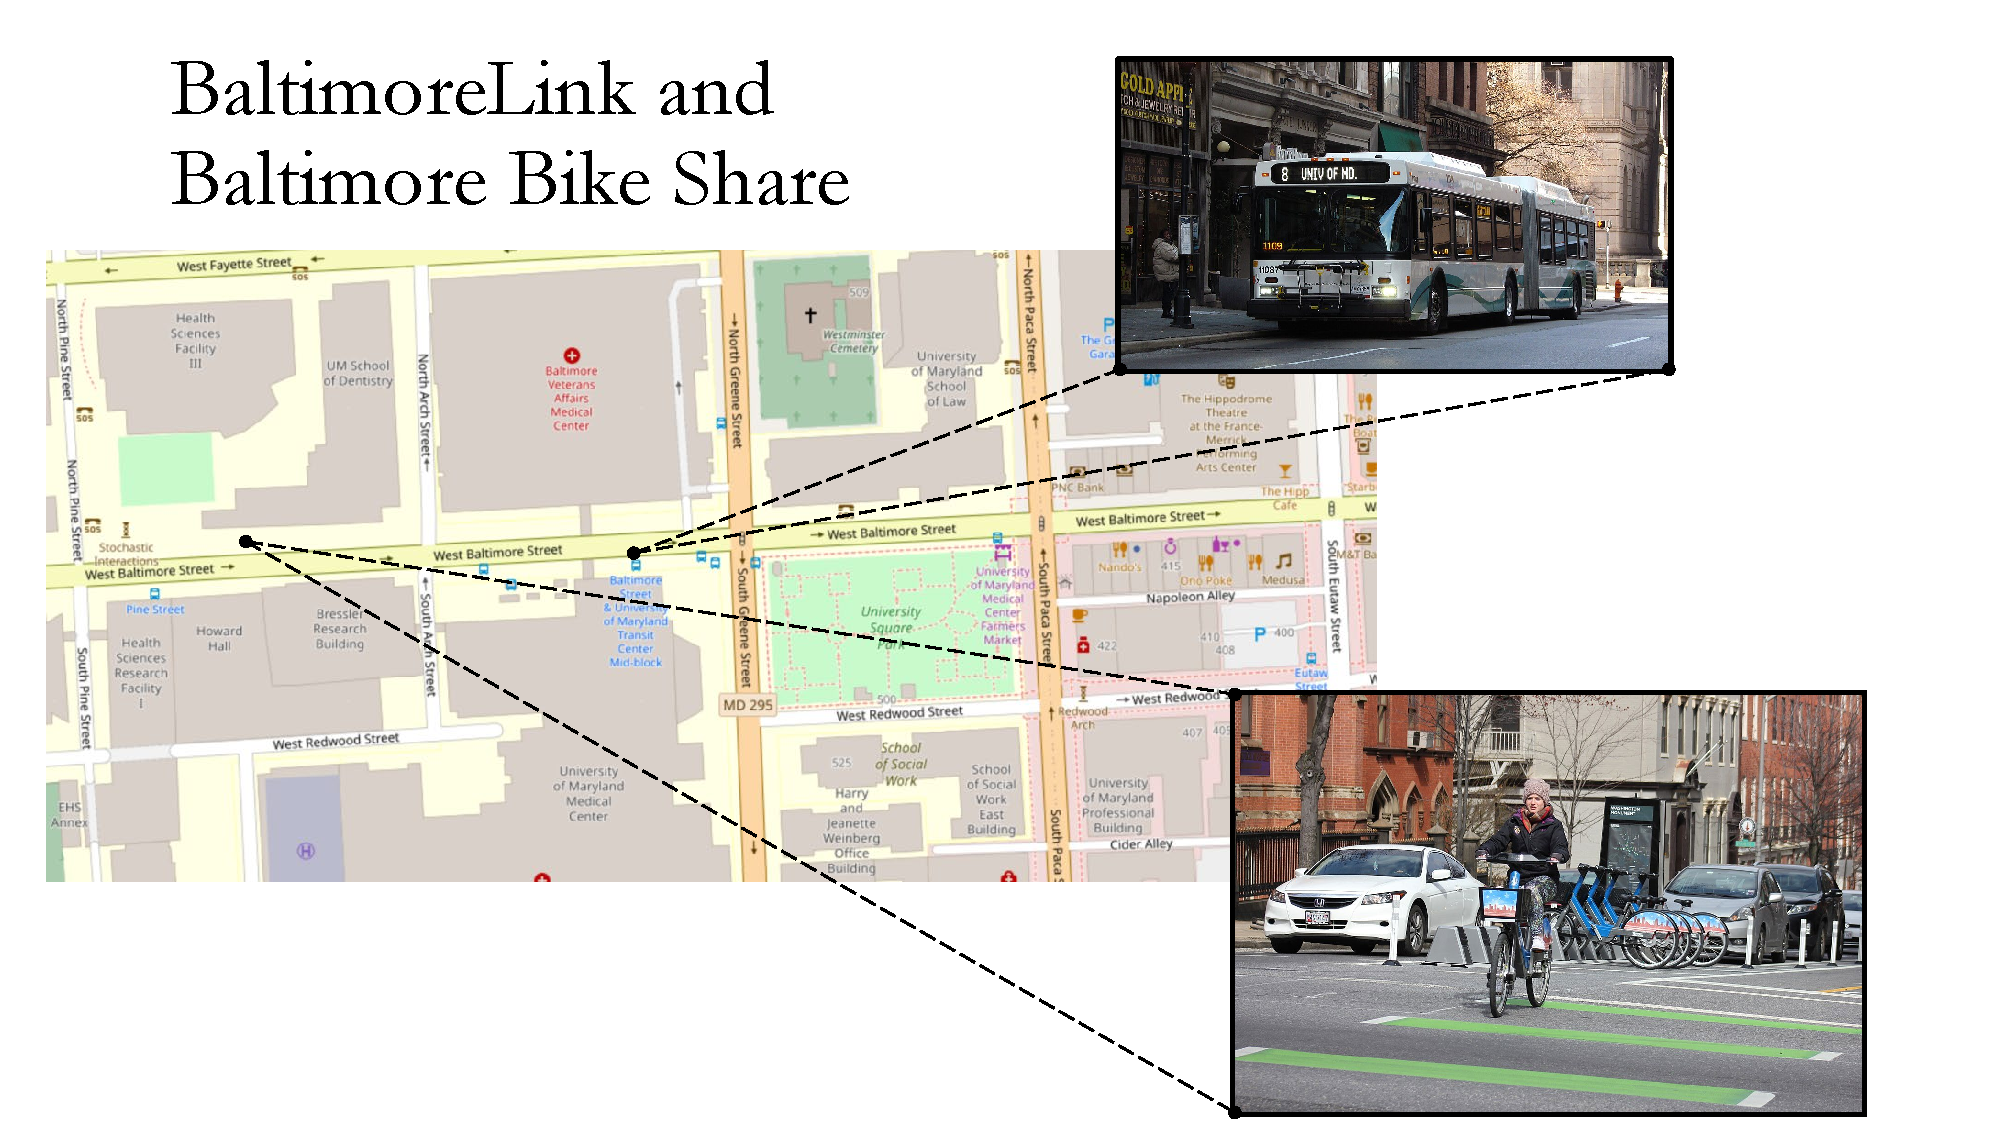
\includegraphics[width=\textwidth]{figures/intro.pdf}
    \caption{巴尔的摩的各种交通:自行车与巴士}
    \label{fig:intro}
\end{figure}

交通网络堪称城市的脉络,关乎着一个城市的发展和居民的生活水平,美国马里兰州巴尔的摩市同样如此。受到原有老化的基础设施和有限的交通选择的影响,巴尔的摩市政府正着眼于重新设计和优化其交通系统,以促进城市发展和利益相关者各方的生活水平和满意度,同时适应未来的需求并确保可持续发展。

\subsection{问题重述}
\label{sec:problem}

根据问题背景信息,我们需要建模巴尔的摩市的交通网络,改善利益相关者们的通勤。主要分为以下任务:

\begin{enumerate}
  \item 根据题目所给数据,建模巴尔的摩市交通网络并将其可视化。
  \item 分析弗朗西斯·斯科特·基桥的倒塌对巴尔的摩的交通系统产生的影响,并分析各个利益相关者的影响。
  \item 选择一个影响公交系统或人行道系统的项目,分析我们的巴尔的摩交通网络模型对其的影响,并分析对各个利益相关者的影响。
  \item 推荐一个最能改善巴尔的摩居民生活的交通网络项目,并对其分析。
\end{enumerate}

\subsection{文献综述}
\label{sec:zongshu}

根据\ref{sec:problem}所提出的要求,我们查找了大量文献。针对分析网络结构中的关键节点的方法主要是基于网络物理结构的中心化方法\citep{ren2014}、度中心算法\citep{zhang2017}、介数中心性算法\citep{bergamini2014}、K-Shell 算法\citep{maji2020}、PageRank 算法\citep{tortosa2021}等。但上述方法都仅是从单一方面寻找反映节点重要程度的因素,并没有考虑到实际问题中各个指标的影响,无法充分挖掘网络隐含的特征,因此关键节点识别结果准确度较低。本文基于这些方法,提出了一种基于节点权重和边权重改进的K-Shell分解算法,并取得了令人兴奋的结果。

\begin{figure}[H]
  \centering
  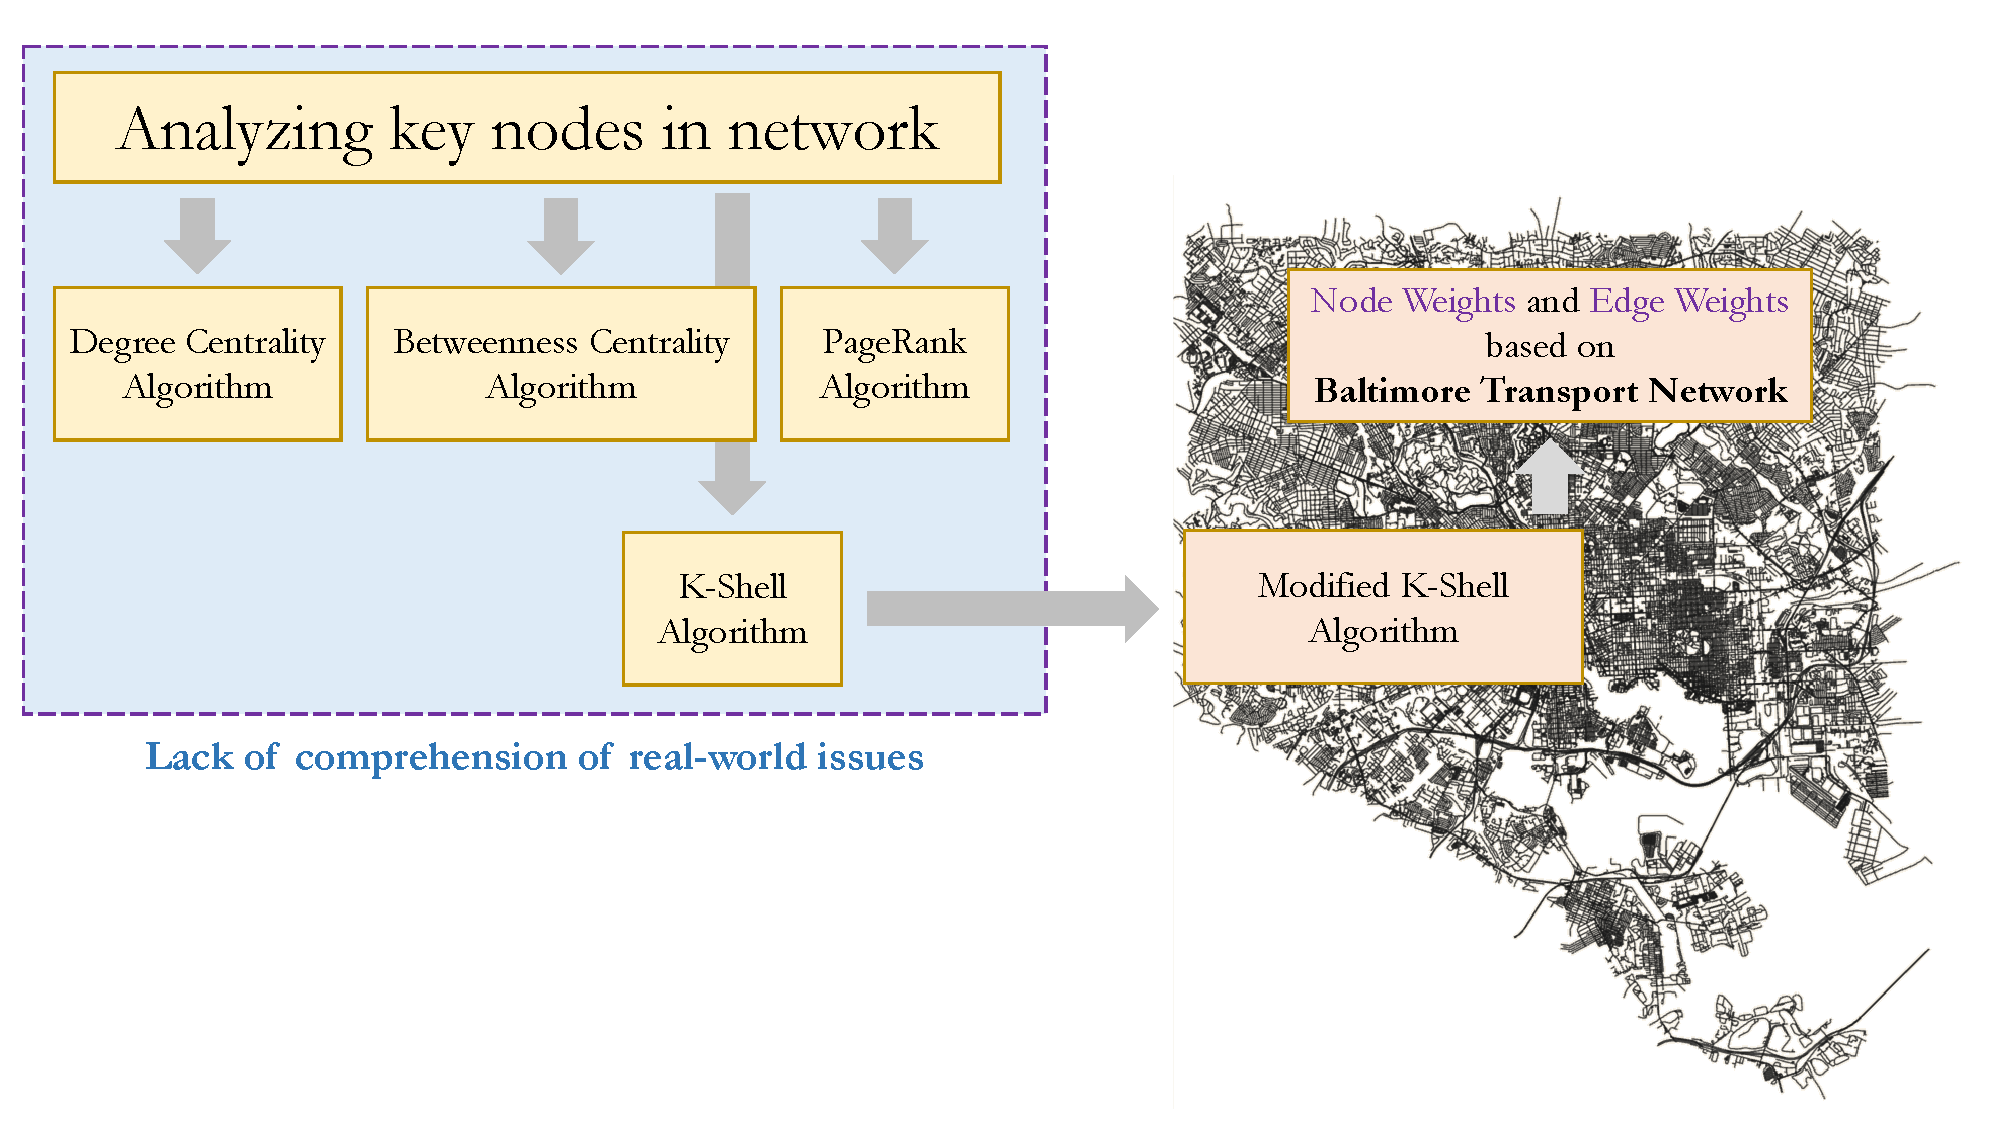
\includegraphics[width=\textwidth]{figures/zongshu.pdf}
  \caption{文献综述思路图}
  \label{fig:zongshu}
\end{figure}


\subsection{我们的工作}

【未完成】

\section{假设}

\begin{enumerate}
    \item 假设公交站点的客流量可以在一定程度上反映附近的人流量,且乘客下车后客流量均匀分配到道路两侧。
    \item 假设巴尔的摩城市中\texttt{access=private}的私有路段不属于城市交通网络的一部分。
    \item 假设在考虑巴尔的摩公交站点线路时,数据集中\texttt{rider\_total}可以充分代表客流量。
\end{enumerate}

\section{符号说明}

\begin{table}[H]
  \centering
  \caption{Symbols and Definitions}
  \label{tab:symbols}
  \begin{tabular}{cl}
    \toprule
    \textbf{Symbol}      & \textbf{Definition} \\
    \midrule
    $d_i^{(w)}$          & Weighted degree of node \\
    $n_i$                & Node weight \\
    $s_i$                & Node score \\
    $\alpha$             & Proportional coefficient of $d_i^{(w)}$ \\
    $\mathrm{score}$     & Evaluation score of the optimized bus route model \\
    $\rho(x,t)$          & Traffic density \\
    \bottomrule
  \end{tabular}
\end{table}

\section{巴尔的摩市交通网络的建模}

\subsection{网络模型的表示}

根据\ref{sec:zongshu},传统方法建立交通网络模型时,大多数仅仅依靠网络的拓扑结构分析节点的重要性,而忽略城市的实际情况,如客流量、气候、地形等重要因素。而我们则提出了一种基于点权重和边权重的K-Shell模型。\textbf{点权重和边权重的比例可代表各方的利益},见表。这不仅考虑了图网络的拓扑结构,而且还考虑了城市的实际情况。我们把城市交通抽象为一个复杂网络 \(G=(V,E)\),其中 \(|V|=N, |E|=M,E\subseteq V\times V\)。
城市中道路的交叉口或断点定义为网络 \(G\) 中的点,记为 \(V=\{v_1, v_2, \ldots, v_N\}\),点的数量记为 \(N\),城市中所有的道路定义为网络 G 中的边,记为 \(E= \{e_1, e_2, \ldots, e_M\}\),边的数量记为 \(M\)。

\subsection{基于节点和边权重改进的K-Shell分解算法}
\label{sec:improvedKshell}

给定一个带有节点和边权重的有向图 \(G = (V, E)\),其中 \(V\) 是节点集合,\(E\) 是边集合。每条边 \(e_{ij} \in E\) 具有权重 \(w_{ij}\),每个节点 \(v_i \in V\) 具有权重 \(n_i\)。

\subsubsection{已知数据的分类}

\begin{figure}[H]
  \centering
  
\includegraphics[width=\textwidth]{figures/data.pdf}
  \caption{已知数据的类型}
  \label{fig:data}
\end{figure}

我们对巴尔的摩数据项可划分为两类,一类描述路网和交点,另一类描述交通流量及其波动。它们当中有些项和节点权重相关,有些项则与边权重相关。可划分如下:

计算点权重的数据,一方面来自节点,比如其经纬度位置 \texttt{X} 和 \texttt{Y}、连接到节点的街道数 \texttt{street\_count}、交叉口类型 \texttt{junction} 等;另一方面来自公交站点的数据,比如站点的位置 \texttt{X} 和 \texttt{Y}、站点的总上下车人数 \texttt{Rider\_Tota}、站点的总乘客累计数 \texttt{Stop\_Rider} 等。

计算边权重的数据,主要来自边,比如其起点终点 \texttt{u} 和 \texttt{v}、车道数 \texttt{lanes}、最大车速 \texttt{maxspeed}、长度 \texttt{length}、服务类型 \texttt{service} 等;还有一些来自各种交通量,比如公交路线的乘车量 \texttt{Distributi}、\texttt{AAWDT}、\texttt{AVMT}、\texttt{AADT} 等;最后,车辆的流向也十分重要,比如方向流量调整系数 \texttt{D-Factor}、高峰小时交通量调整系数 \texttt{K-Factor} 等。

\subsubsection{改进的K-Shell分解算法}

\begin{table}[H]
  \centering
  \label{tab:improvedKshell}
  \begin{tabular}{@{}p{0.95\textwidth}@{}}
  \toprule
  \textbf{Algorithm 1: The Improved K-Shell Decomposition Algorithm for Key Node Identification} \\ 
  \midrule
  \textbf{Input:} Graph network \(G=(V, E)\) \\
  \textbf{Output:} Node importance ranking result \\
  \textbf{Step 1:} Calculate the initial weighted degree of each node \(d_i^{(w)}=\sum_{j\in N(i)}w_{ij}\), where \(N(i)\) represents the set of adjacent nodes of node \(i\). \\
  \textbf{Step 2:} For each node \(i\), calculate the score \(s_i\) given by a certain stakeholder using the formula \(s_i = \alpha d_i^{(w)}+(1 - \alpha)n_i\). \textbf{Here, \(\alpha\) is a regulatory parameter, which can reflect the priority requirements of different stakeholders for node weights and edge weights in the transportation network. See \ref{sec:alpha}.} Both \(d_i^{(w)}\) and \(n_i\) are normalized using the min - max normalization method. \\
  \textbf{Step 3:} Iteratively remove nodes with low scores
  \begin{itemize}
      \item Find the set \(S\) of nodes with the lowest comprehensive scores in the current graph.
      \item Assign these nodes to the current K-Shell layer and remove them from the graph.
      \item Update the weighted degrees of the remaining nodes:
      \begin{equation}
          d_j^{(w)}=d_j^{(w)}-w_{ij}\quad\text{for all }j\in N(i)
      \end{equation}
  \end{itemize}
  \textbf{Step 4:} Repeat the above steps for the remaining graph until all nodes are assigned to a certain K-Shell layer. \\ \bottomrule
  \end{tabular}
\end{table}

\subsection{节点和边权重的确定}

\subsubsection{点权重的确定}

点权重主要考虑政府方面,当某节点的人流量增大后,可以促进当地的经济发展,推动旅游业,增大企业活力。因此点权重我们以节点的净流量为标准。

根据假设1,乘客上下车方向均匀分配,有:

\begin{itemize}
  \item 上车乘客以 \(\frac{U_{uv}}{2}\) 的比例分别从节点 \(u\) 和 \(v\) 进入道路,\(U_{uv}\) 表示在该站点进入道路的乘客总数
  \item 下车乘客以 \(\frac{D_{uv}}{2}\) 的比例分别前往节点 \(u\) 和 \(v\) ,\(D_{uv}\) 表示在该站点离开道路的乘客总数
\end{itemize}

我们定义某节点 \(u\) 的相邻边集合为 \(\mathcal{E}\),首先计算节点流出量(从节点离开的乘客)和节点流入量(到达节点的乘客):

\begin{equation}
  \begin{cases} 
  \text{Outflow}(i) = \dfrac{1}{2} \sum_{(i, j) \in \mathcal{E}} U_{ij} \\
  \text{Inflow}(i) = \dfrac{1}{2} \sum_{(j, i) \in \mathcal{E}} D_{ji} 
  \end{cases}
\end{equation}

最后我们计算节点净流量来代表节点权重:

\begin{equation}
\text{Net}(i) = \text{Inflow}(i) - \text{Outflow}(i)=\frac{1}{2} \sum_{(i, j) \in \mathcal{E}} U_{ij}-\frac{1}{2} \sum_{(j, i) \in \mathcal{E}} D_{ji}
\end{equation}

\subsubsection{边权重确定}

边权重主要由居民、游客、过境旅客的通行时间来衡量,我们从数据文件中收集出与边权重相关指标:道路类型、道路段上车道数量、道路上的最大速度限制、道路是否为单向、道路长度、道路宽度、车道数等,由此建立以下模型:

BPR 函数描述了行程时间与交通流量的关系:

\begin{equation}
t = t_0 \left(1 + \alpha \left(\frac{V}{C}\right)^\beta\right)
\end{equation}

其中 \(t\) 代表行程时间, \(t_0\) 为自由流时间(无拥堵时的行程时间),\(V\) 表示交通流量(如 AADT,年度平均日交通量), \(C\) 表示道路通行能力,而\(\alpha, \beta\) 为经验参数(通常取 \(\alpha=0.15 , \beta=4\) )\cite{hamdouch2014} \cite{gao2004}。

根据 BPR 函数,我们可以得出,实际速度 \(v\) :

\begin{equation}
v = \frac{L}{t} = \frac{L}{t_0 \left(1 + \alpha \left(\frac{V}{C}\right)^\beta\right)},
\end{equation}

其中 \(L\) 为道路长度。自由流速度 \(v_0 = \frac{L}{t_0}\),因此:

\begin{equation}
v = \frac{v_0}{1 + \alpha \left(\frac{V}{C}\right)^\beta}.
\end{equation}

此外,通行能力 \(C\) 受车道数\texttt{lanes}和道路功能分类\texttt{Functional Class}(州际公路、主干道、地方道路)影响。最后我们引入其他调整因子

\begin{itemize}
  \item 道路特征修正
    \begin{itemize}
      \item 隧道\texttt{tunnel=yes}:速度降低15\%,即 \(v_{\text{final}} = v \times 0.85\)。
      \item 桥梁\texttt{bridge=yes}:速度降低10\%,即 \(v_{\text{final}} = v \times 0.9\)。
      \item 单向道路\texttt{oneway=True}:速度提高5\%,即 \(v_{\text{final}} = v \times 1.05\)。
    \end{itemize}
  \item 车道数影响
    \begin{itemize}
      \item 车道数越多,通行效率越高:\(C = C_{\text{base}} \times \text{lanes}\)。 
    \end{itemize}
\end{itemize}

综合所有因素后,我们可以得出:

\begin{equation}
v_{\text{final}} = \frac{v_0}{1 + \alpha \left(\frac{\text{AADT}}{C}\right)^\beta} \times f_{\text{tunnel}} \times f_{\text{bridge}} \times f_{\text{oneway}},
\end{equation}

其中:

\begin{itemize}
  \item \(f_{\text{tunnel}} = 1 - 0.15 \times \text{is\_tunnel}\),\(\text{is\_tunnel}\in\{0,1\}\)
  \item \(f_{\text{bridge}} = 1 - 0.1 \times \text{is\_bridge}\),\(\text{is\_bridge}\in\{0,1\}\)
  \item \(f_{\text{oneway}} = 1 + 0.05 \times \text{is\_oneway}\),\(\text{is\_oneway}\in\{0,1\}\)
\end{itemize}

最终,边的权重由通行时间来确定:

\begin{equation}
t=\frac{L}{v_{final}},
\end{equation}

其中,\(L\)表示道路长度。

\subsection{由利益相关方确定\(\alpha\)}
\label{sec:alpha}

我们再分析巴尔的摩市的情况后,把利益相关方划分为以下三个主要的需求不同的群体,并根据他们的自身工作或生活特性确定他们的 \(\alpha\),如\ref{tab:stakeholder_data}所示:

\begin{table}[H]
  \centering
  \caption{Stakeholder Data}
  \label{tab:stakeholder_data}
  \begin{tabular}{@{}lccc@{}}
    \toprule
    \textbf{Stakeholder Groups} & \textbf{Main Concerns} & \textbf{$\alpha$} & \textbf{GDP Proportion} \\
    \midrule
    Local Residents & Convenience & $\alpha_1 = 0.7$ & \(GDP_1\) = 35.55\% \cite{mdba} \\
    Freight Enterprises & Transportation Efficiency & $\alpha_2 = 0.1$ & \(GDP_2\) = 60.54\% \cite{gdpa}\\
    Tourists & Balanced Demands & $\alpha_3 = 0.5$ & \(GDP_3\) = 3.91\% \cite{aboutus} \\
    \bottomrule
  \end{tabular}
\end{table}

由此,我们可建立巴尔的摩综合网络重要性比例系数:
\begin{equation}
  \alpha_{\text{总}}=\sum_{i=1}^{n}\omega_i\cdot\alpha_i,\quad i=1,2,3,
\end{equation}
其中,\(\omega_i\) 为利益相关者群体的权重,由 GDP 占比确定,即\(w_i=GDP_i\)。

带入计算后得到最终权重为:
\begin{equation}
  \alpha_{\text{总}}=0.32534
\end{equation}

\subsection{数据预处理}

\subsubsection{数据筛选}

由于题目所给数据地理范围为巴尔的摩都会区,远大于巴尔的摩市区的范围,所以我们首先根据经纬度筛选出巴尔的摩市范围内的数据,筛选结果如表所示:

\begin{table}[H]
  \centering
  \caption{Data Statistics Before and After Filtering}
  \label{tab:data_filtering_stats}
  \begin{tabular}{@{}lcc@{}}
      \toprule
      \textbf{Data Table} & \textbf{Before Filtering} & \textbf{After Filtering} \\
      \midrule
      edge\_all.csv & 565,495 entries & 201,003 entries \\
      edge\_drive.csv & 91,227 entries & 29,309 entries \\
      \bottomrule
  \end{tabular}
\end{table}

\subsubsection{缺失值填充: 快速填充算法确定AADT}

AADT data is only collected on roads with bus stops, while other roads lack such data. However, the time complexity of directly using the shortest - distance method to fill the missing AADT values is too high. Therefore, we use the following fast - filling algorithm to determine the AADT values of all roads.

\begin{table}[H]
  \centering
  \label{tab:AADTFilling}
  \begin{tabular}{@{}p{0.95\textwidth}@{}}
  \toprule
  \textbf{Algorithm 2: Fast Filling Algorithm for AADT Values of All Roads} \\ 
  \midrule
  \textbf{Step 1:} Assign the AADT value of all edges to 0, and update the AADT values of edges with bus stops. \\
  \textbf{Step 2:} Traverse the edges that have been assigned AADT values. For each such edge \(e_i\), traverse the edges \(e_j\) connected to it, and add the AADT value of \(e_i\) to the AADT list of \(e_j\). \\
  \textbf{Step 3:} Calculate the average value of the AADT list of \(e_j\) obtained in Step 2, and use it as the AADT value of \(e_j\). \\
  \textbf{Step 4:} Repeat Step 2 and Step 3 until there is no edge with an AADT value of 0 in the entire network. \\ \bottomrule
  \end{tabular}
\end{table}


\begin{figure}[H]
    \centering
    \subfigure[]{
    \begin{minipage}[t]{0.33\linewidth}
    \centering
    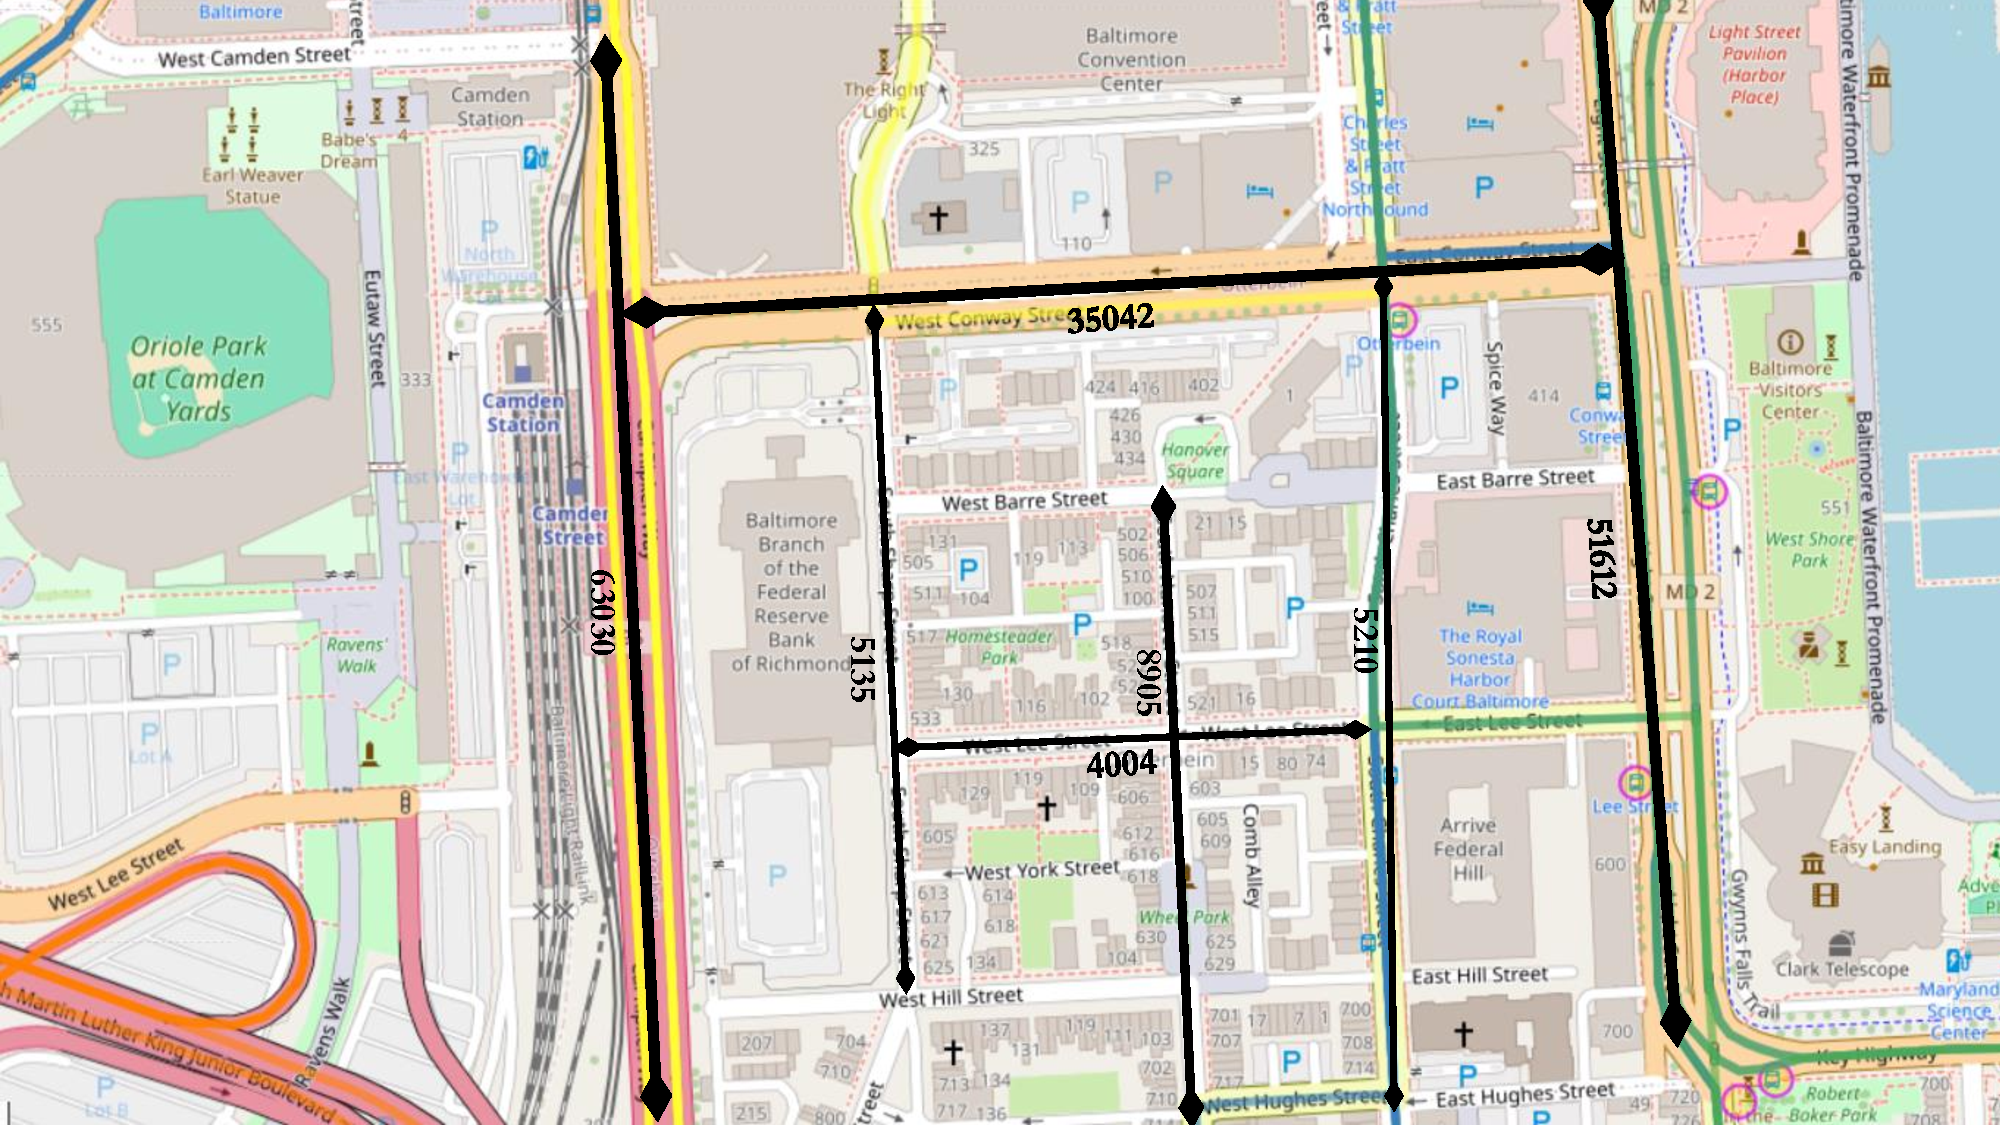
\includegraphics[width=\linewidth]{figures/topo1.pdf}
    \end{minipage}%
    % \label{fig:}%
    }%
    \subfigure[]{
    \begin{minipage}[t]{0.33\linewidth}
    \centering
    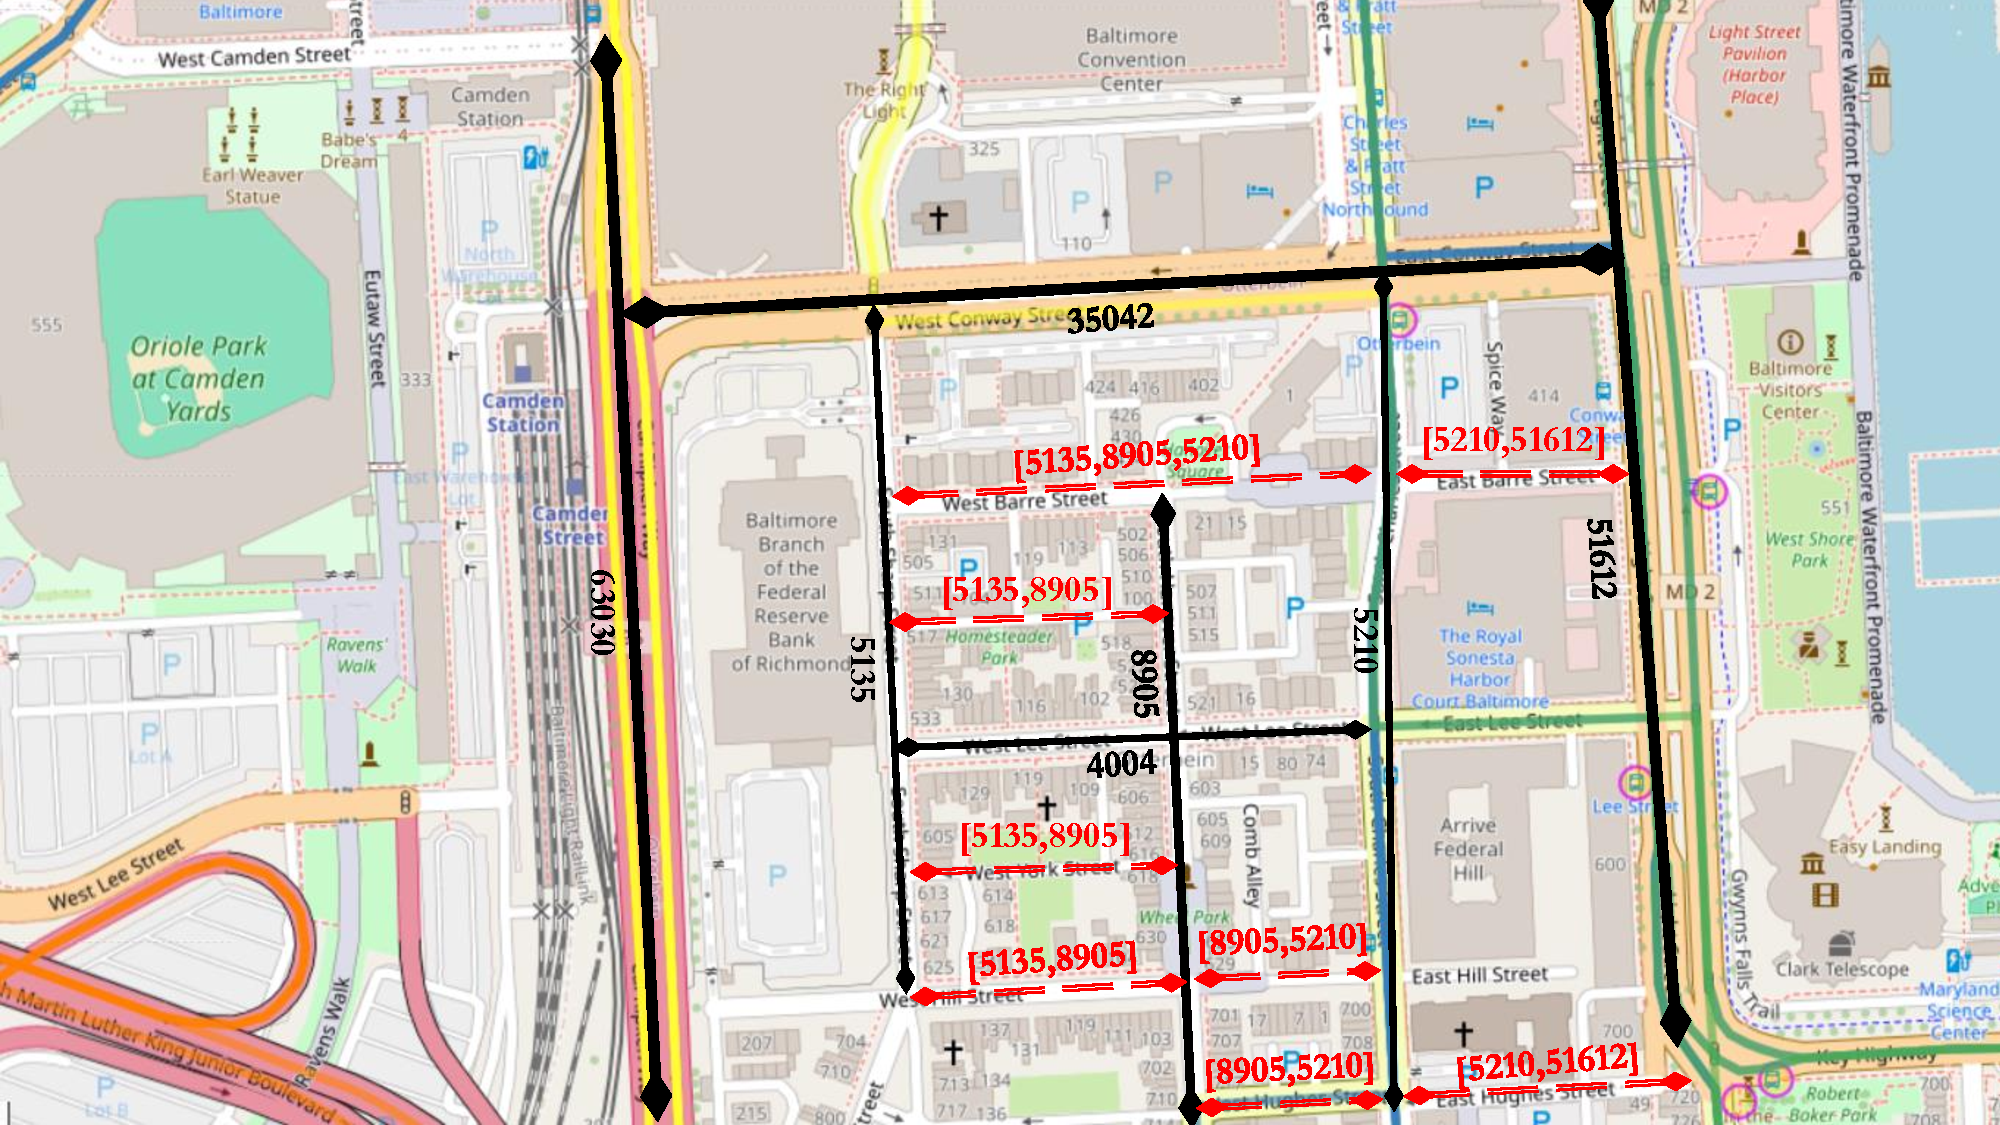
\includegraphics[width=\linewidth]{figures/topo2.pdf}
    \end{minipage}%
    % \label{fig:}%
    }%
    \subfigure[]{
        \begin{minipage}[t]{0.33\linewidth}
        \centering
        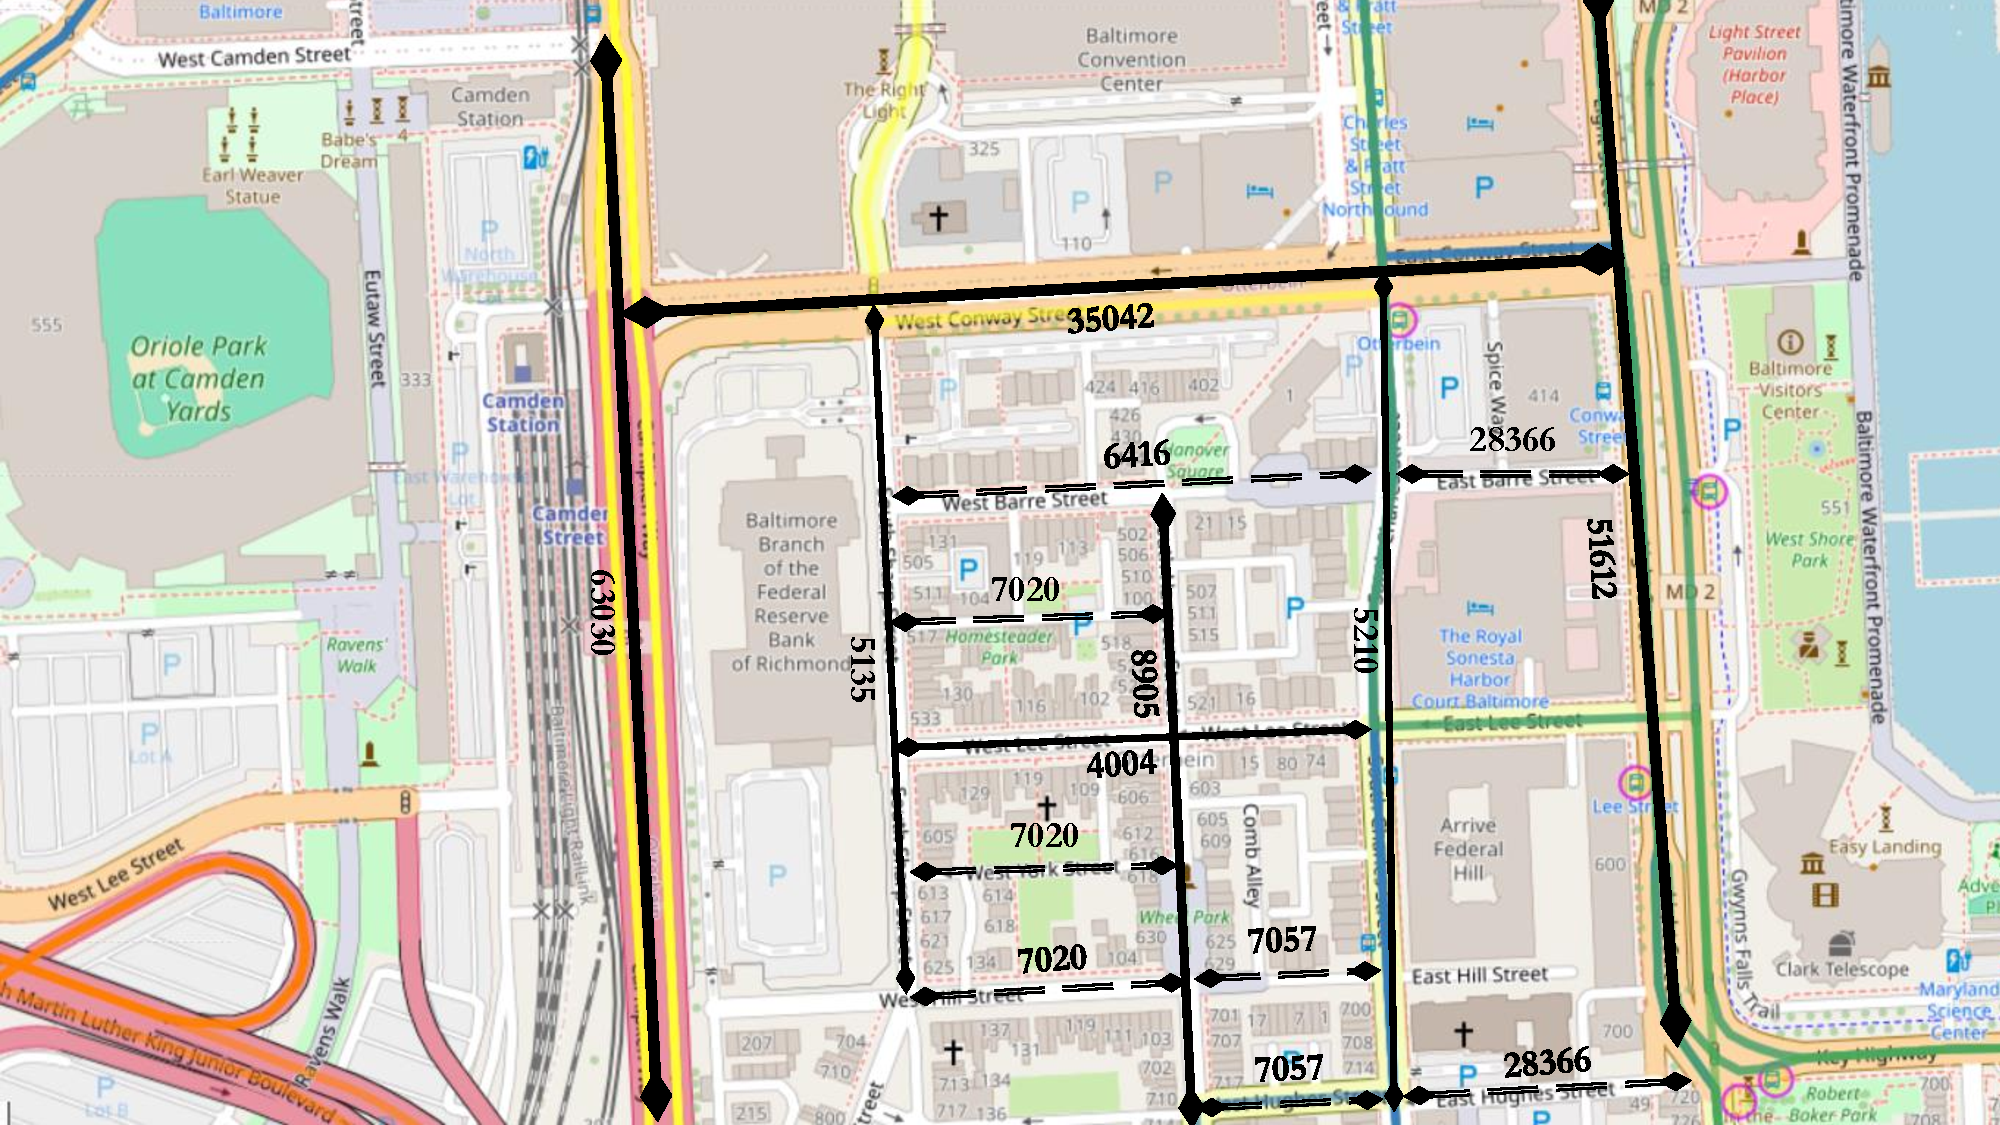
\includegraphics[width=\linewidth]{figures/topo3.pdf}
        \end{minipage}%
    % \label{fig:}%
    }%
    \caption{AADT填充示例}
    \label{fig:aadt}
\end{figure}

\subsection{巴尔的摩市交通网络的可视化}

我们根据巴尔的摩城市交通网络模型,计算出重要性在前1000名的节点,并可视化,结果如下图所示:

\begin{figure}[H]
  \centering
  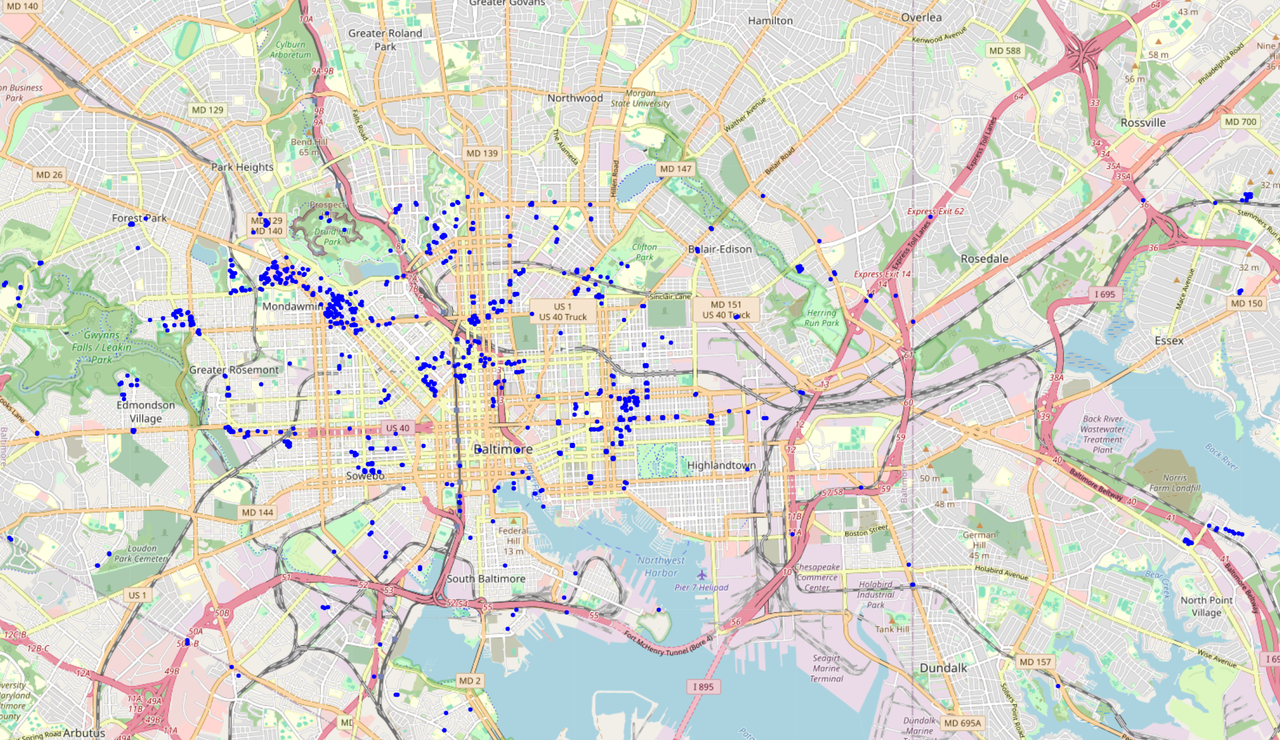
\includegraphics[width=\textwidth]{figures/vis.png}
  \caption{前1000名重要的节点可视化}
  \label{fig:vis}
\end{figure}

\section{问题1:交通网络模型应用于弗朗西斯·斯科特·基桥倒塌事件}

2024年3月26日,一起交通事故导致弗朗西斯·斯科特·基大桥坍塌,造成交通瘫痪。我们团队根据上文的巴尔的摩市交通网络模型,分析大桥坍塌前后的节点重要性变化,发现在大桥坍塌后,邻近道路节点(如I-95隧道、I-895隧道)的重要性评分上升,成为替代路径的拥堵热点。我们分别计算出大桥坍塌前后巴尔的摩市交通网络的节点重要性评分,然后借此画出大桥坍塌后节点重要性提升百分比热力图,结果显示I-895隧道重要性提升最明显,在63.7\%左右,I-95隧道次之,约为47.2\%,城市中绕行的道路平均也有10\%~20\%的提升。这也说明了巴尔的摩城市交通网络中的问题:路径冗余不足、多模式衔接断裂。

\begin{figure}[H]
  \centering
  \subfigure[Before Collapse]{
  \begin{minipage}[t]{0.3\linewidth}
  \centering
  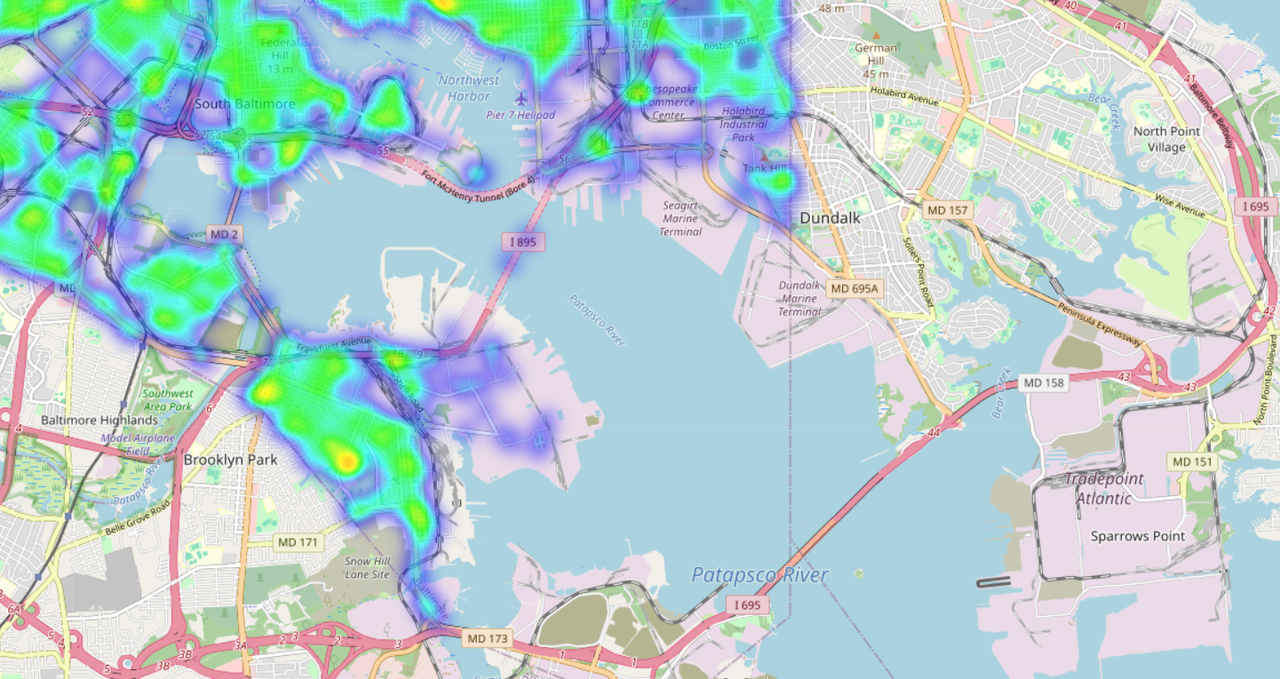
\includegraphics[width=\linewidth]{figures/heatmapbefore.png}
  \end{minipage}%
  % \label{fig:}%
  }%
  \subfigure[After Collapse]{
  \begin{minipage}[t]{0.7\linewidth}
  \centering
  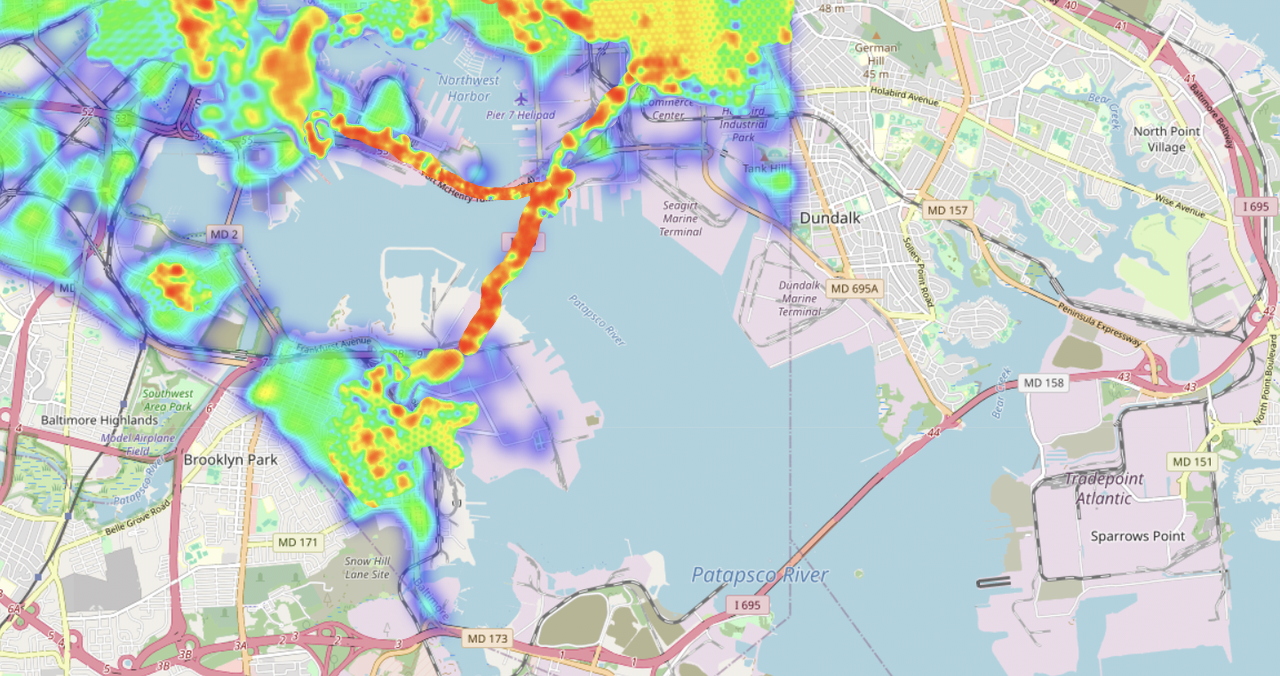
\includegraphics[width=\linewidth]{figures/heatmap.png}
  \end{minipage}%
  % \label{fig:}%
  }%
  \caption{Heatmap of Importance Increase}
  \label{fig:heatmap}
\end{figure}

然后,我们根据本地居民、货运企业、游客三种不同利益者的 $\alpha$ 值分别计算巴尔的摩城市交通网络节点重要性提升情况,结果如下表所示。我们发现,在弗朗西斯·斯科特·基大桥坍塌前后,本地居民利益者的巴尔的摩交通网络节点重要性变化幅度很少,这是因为本地居民活动范围相对固定,一般不会去对岸。而游客次之,这是因为他们去对岸的可能性比本地居民大。货运企业最高,因为他们要频繁来往两岸。此外,值得注意的是,由于1-895隧道和1-95隧道可能对来往车辆有着限制,他们不得不在城市中绕行,所以城市绕行的重要性提升百分比相对较高。

\section{问题2:交通网络模型应用于优化公交线路}

\subsection{基于 PCA 的特征权重分析}

\subsubsection{数据选择与处理}

在公交站点数据集\texttt{Bus\_Stops.csv}中,我们需要对公交站点的特征进行分析,确定每个特征对聚类结果的贡献权重,并基于这些权重进行聚类。经过筛选,我们除去了一些无意义、含义重复、数据单一的列后,选择以下数据指标:
类别型变量\texttt{Mode}、\texttt{Shelter},数值型变量\texttt{X}、\texttt{Y}、\texttt{Rider\_Total}、\texttt{Stop\_Rider}。

由于类别型特征无法直接用于 PCA,我们首先对其进行 One-Hot 编码,然后通过 PCA 分析确定每个特征的权重。PCA 对数据的尺度敏感,因此需要对数值型特征进行标准化。

\subsubsection{主成分分析}

标准化后的数据矩阵为 $\mathbf{X} \in \mathbb{R}^{n \times p}$,其中 $n$ 是样本数,$p$ 是特征数。协方差矩阵 $\mathbf{C}$ 的计算公式为:

\begin{equation}
\mathbf{C} = \frac{1}{n - 1} \mathbf{X}^T \mathbf{X}
\end{equation}

对协方差矩阵 $\mathbf{C}$ 进行特征值分解:
\begin{equation}
\mathbf{C} = \mathbf{V} \mathbf{\Lambda} \mathbf{V}^T
\end{equation}
其中$\mathbf{V}$ 是特征向量矩阵,$\mathbf{\Lambda}$ 是特征值对角矩阵。

主成分 $\mathbf{P}$ 是原始数据在特征向量方向上的投影:
\begin{equation}
\mathbf{P} = \mathbf{X} \mathbf{V}
\end{equation}

每个主成分的方差贡献率为:
\begin{equation}
\text{Explained Variance Ratio}_i = \frac{\lambda_i}{\sum_{j = 1}^p \lambda_j}
\end{equation}
其中 $\lambda_i$ 是第 $i$ 个特征值。

\subsubsection{特征权重计算}

对于类别型特征,如 \texttt{Mode}和\texttt{Shelter},我们使用 One-Hot 编码将其转换为二进制向量。假设类别型特征 $\mathbf{C}$ 有 $k$ 个取值,则 One-Hot 编码后的特征矩阵为:
\begin{equation}
\mathbf{C}_{\text{encoded}} \in \mathbb{R}^{n \times k}
\end{equation}

将标准化后的数值型特征 $\mathbf{X}_{\text{scaled}}$ 和 One-Hot 编码后的类别型特征 $\mathbf{C}_{\text{encoded}}$ 合并:
\begin{equation}
\mathbf{X}_{\text{processed}} = [\mathbf{X}_{\text{scaled}}, \mathbf{C}_{\text{encoded}}]
\end{equation}

对合并后的数据 $\mathbf{X}_{\text{processed}}$ 进行 PCA 分析,得到每个主成分的方差贡献率 $\text{Explained Variance Ratio}_i$。将 One-Hot 编码后的特征的方差贡献合并回原始类别。假设原始类别型特征 $\mathbf{C}$ 的 One-Hot 编码列对应的方差贡献为 $\text{Explained Variance Ratio}_j$,则原始类别的权重为:
\begin{equation}
\text{Weight}_i = \sum_{j \in \text{Category}_i} \text{Explained Variance Ratio}_j
\end{equation}

将权重归一化,使其总和为 1:
\begin{equation}
\text{Normalized Weight}_i = \frac{\text{Weight}_i}{\sum_{j = 1}^p \text{Weight}_j}
\end{equation}

至此,我们计算出了所示数据的权重,结果如下:

\begin{table}[H]
  \centering
  \caption{Data Meanings and Their Weights}
  \label{tab:data_weights}
  \begin{tabular}{@{}lcc@{}}
      \toprule
      \textbf{Data Meaning} & \textbf{Variable} & \textbf{Weight} \\
      \midrule
      Total Number of Riders & \texttt{Rider\_Tota} & 0.62830 \\
      Total Cumulative Number of Riders at Stops & \texttt{Stop\_Rider} & 0.21777 \\
      Transportation Mode Type (e.g., bus) & \texttt{Mode} & 0.03646 \\
      Whether There is a Passenger Shelter & \texttt{Shelter} & 0.00093 \\
      The Service Type of Bus & \texttt{Routes\_Ser} & 0.11650 \\
      \bottomrule
  \end{tabular}
\end{table}

\subsection{基于K-Prototypes的公交站点聚类}

K-Prototypes 算法是一种能够同时处理数值型和类别型数据的聚类方法。我们的数据集包含数值型特征和类别型特征,完全符合 K-Prototypes 算法的要求。此外,我们在\ref{tab:data_weights}中通过 PCA 分析计算了每个特征的权重贡献,这些权重将用于优化聚类过程。

K-Prototypes 与 K-means 算法不同的是,K-Prototypes 算法不仅可以通过欧式距离计算数值类型的相似度,还可以通过汉明距离计算类别类型相似度。

我们对巴尔的摩市公交站点数据进行聚类,多次选取不同的 k 值后,发现 k=5时效果比较理想,聚类可视化结果如下图所示:

\begin{figure}[H]
  \centering
  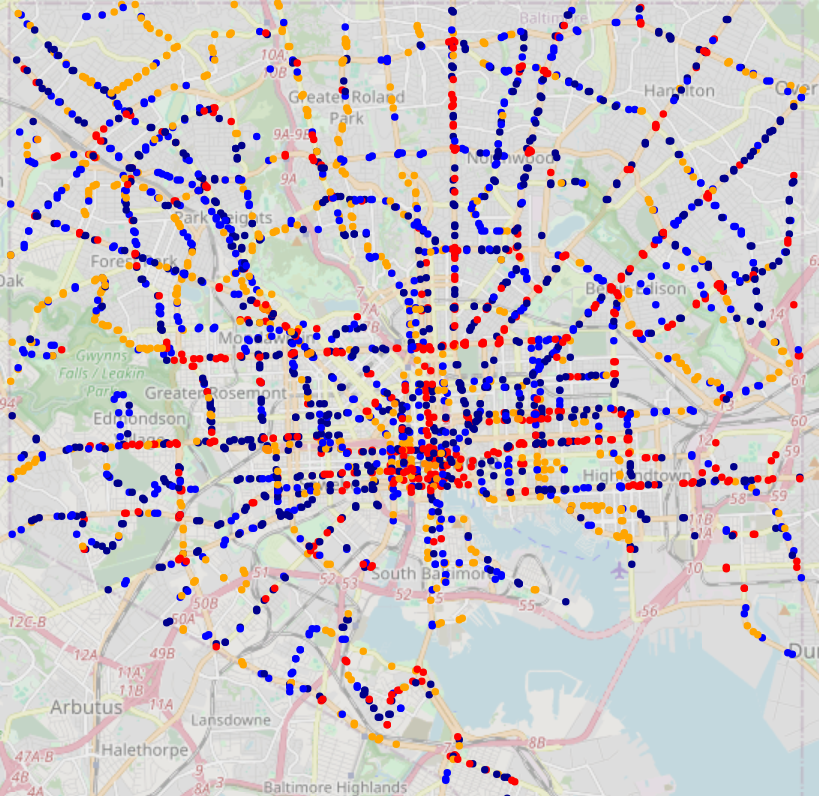
\includegraphics[width=\textwidth]{figures/cluster.png}
  \caption{公交站点聚类可视化}
  \label{fig:cluster}
\end{figure}

观察聚类结果图我们发现:重要性最高的站点很大程度上集中在市中心部分,分布在繁忙的交通线路上。而重要性低的站点大多集中在距离市中心偏远的地区,分布在人流量少的交通线路上。因此,我们考虑选取重要性高的站点集中所在区域进一步分析。

\subsection{基于聚类结果的公交线路优化}

我们抽离出聚类结果中的一块进行分析,尝试为该区域增加公交线路规划。为此我们计算出每个站点对应的分数,在分数高的地方增加公交线路。除了第四节中的节点权重外,针对公交线路,我们还应关注客流量和公交线路数量对分数的影响:客流量越大,越应增加线路;而公交线路越少,越应增加线路。分数具体计算公式如下\footnote{根据假设3,客流量为\texttt{Rider\_Tota} ,公交线路数量为 \texttt{Routes\_Ser} 列表的长度。}:

\begin{equation}
score=\dfrac{\text{客流量}\times \text{站点两侧节点重要性平均值}}{\text{公交线路数量}}
\end{equation}

因为多家医院与大学的地理分布,我们认为在红线部分增加公交线路是最优的,如\ref{fig:busroute}所示。

\begin{figure}[H]
  \centering
  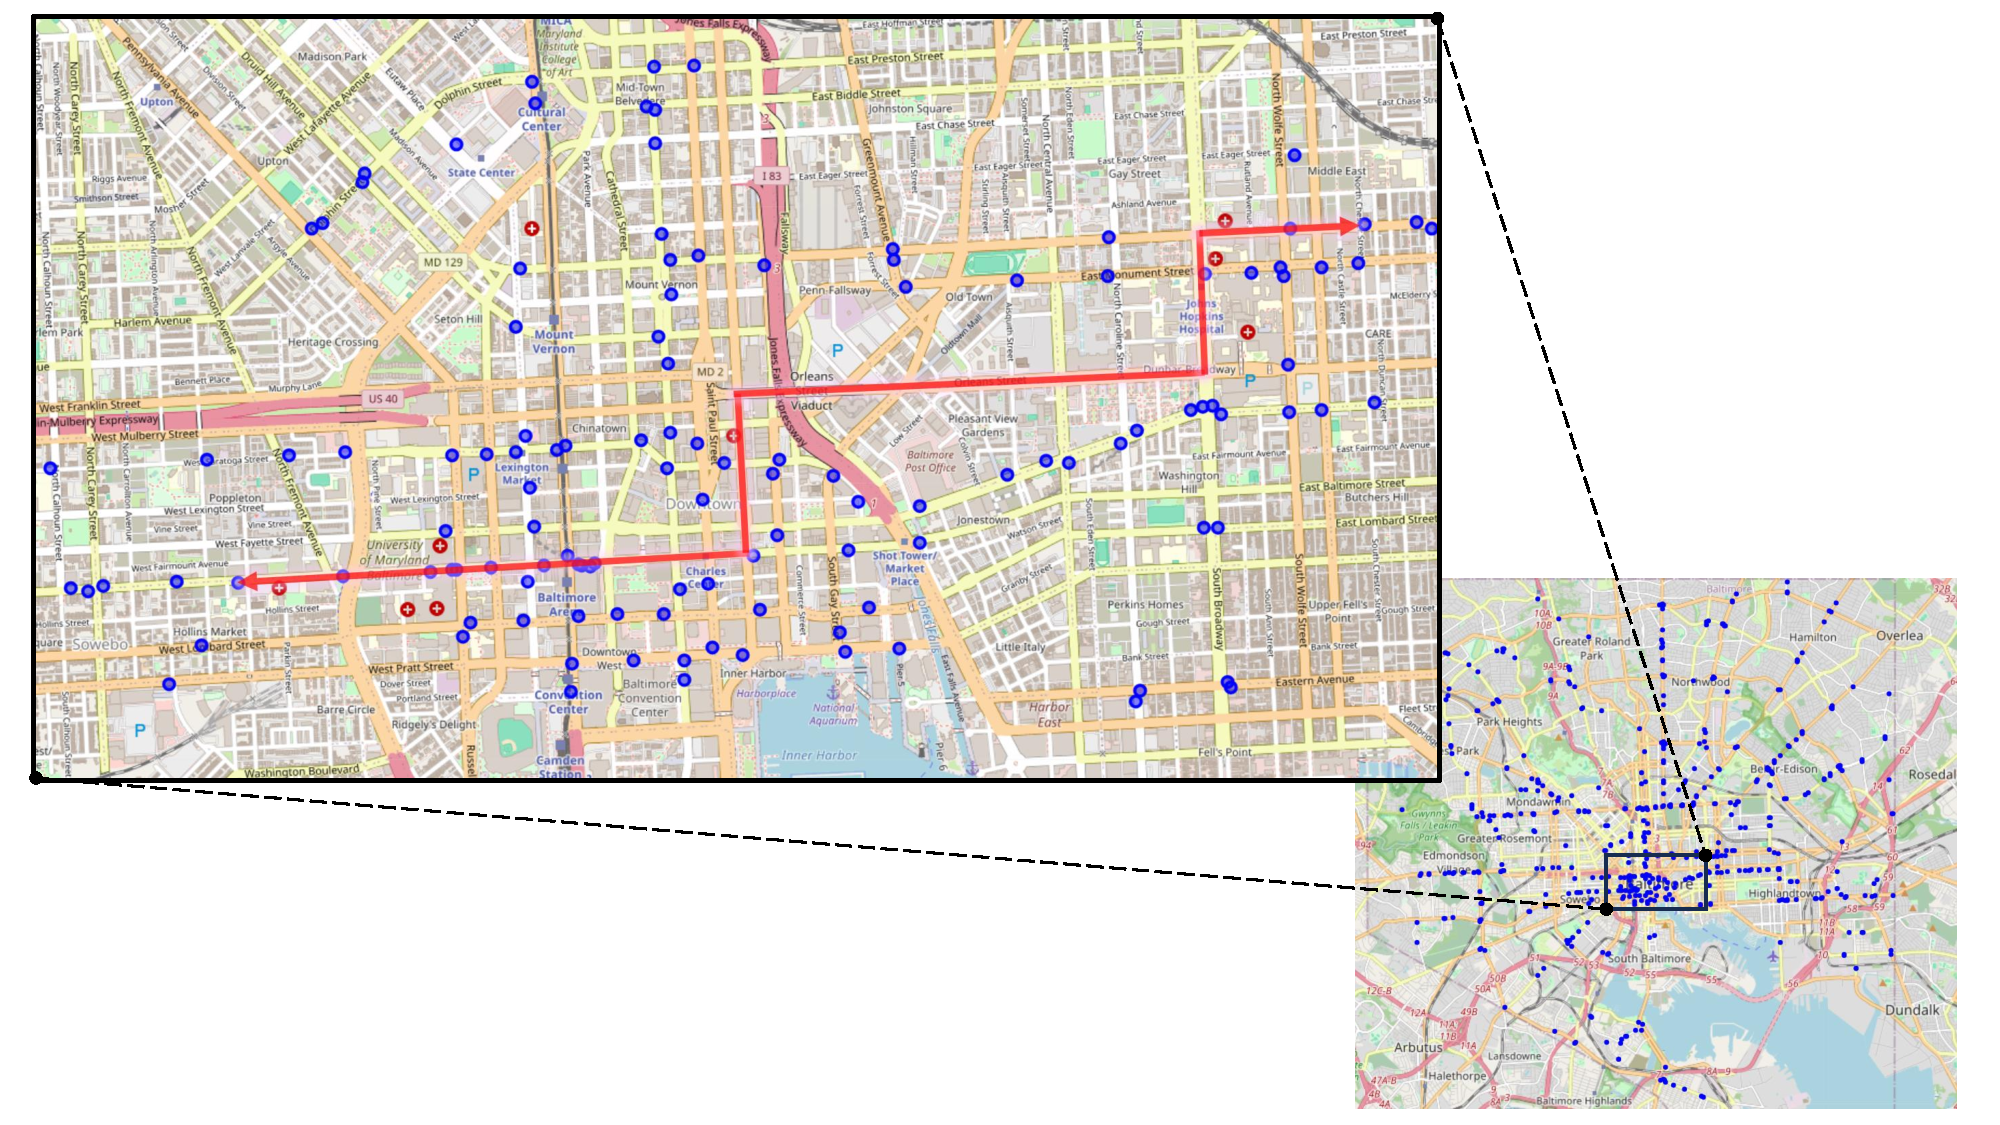
\includegraphics[width=\textwidth]{figures/busroute.pdf}
  \caption{公交线路优化规划}
  \label{fig:busroute}
\end{figure}

\subsection{对周边地区利益相关者的影响}

在地图中标注红线的地方新增公交线路后,极大地方便了周边居民的日常出行,同时也显著提升了旅客的出行体验;同时降低了大学学生等居民驾车出行的意愿,为货运公司提供了更便捷的物流通道。这一改进不仅加强了区域内的交通网络连接,还促进了当地经济的发展,使得居民、旅客以及企业均能从中受益。

\section{问题3:巴尔的摩交通网络的拥堵管理策略}

\subsection{巴尔的摩市的交通隐患}

城市的交通网络拥堵一直是巴尔的摩市的安全隐患,它不仅可能导致了交通事故发生概率的增加,而且交通不便的地区也可能因警力难以快速到达而导致犯罪率上升,此外,人流密集的地方也可能发生踩踏事故,也容易发生盗窃、抢劫等犯罪。为此我们团队设计了一套巴尔的摩交通网络的拥堵管理策略,类比计算机网络领域的拥塞控制算法,分阶段的动态调整信号灯周期和交警数量。

\subsection{交通拥堵的指数模型及拥堵管理策略}

According to the classical LWR model to describe the traffic density $\rho(x,t)$, we have:
\begin{equation}
\frac{\partial \rho}{\partial t} + \frac{\partial}{\partial x} \left( \rho v(\rho) \right) = 0\Rightarrow v(\rho) = v_{\text{free}} \left( 1 - \frac{\rho}{\rho_{\text{max}}} \right)
\end{equation}
where $\rho(x,t)$ is the traffic flow density, $v(\rho)$ is the traffic flow speed, and $\rho_{\text{max}}$ is the road - carrying capacity.

Considering that the importance of the node $w_i$ weakens the local traffic capacity:
\begin{equation}
\rho_{\text{max},i} = \rho_{\text{base}} \cdot \left( 1 - \alpha w_i \right)
\end{equation}

In the local road section (near node $i$), ignoring the spatial derivative term, the LWR equation degenerates into the Logistic equation:
\begin{equation}
\frac{d\rho_i}{dt}=k_i\rho_i\left(1-\frac{\rho_i}{\rho_{\max,i}}\right)
\end{equation}

Considering that the higher the importance of the node, the faster the congestion may spread. Define the modified growth rate:
\begin{equation}
k_i=k_{\mathrm{base}}\cdot(1+\beta w_i)
\end{equation}

Substituting it into the above equation, we get:
\begin{equation}
\frac{d\rho_i}{dt} = k_{\text{base}} (1 + \beta w_i) \rho_i \left( 1 - \frac{\rho_i}{\rho_{\text{base}} (1 - \alpha w_i)} \right)
\end{equation}

Solving the above equation by the method of separation of variables:
\begin{equation}
\rho_i(t) = \frac{\rho_{\text{max},i}}{1 + e^{-k_{\text{base}} (1 + \beta w_i) t} \cdot \left( \frac{\rho_{\text{max},i}}{\rho_{i,0}} - 1 \right)}
\end{equation}

When $\rho_i \ll \rho_{\text{max},i}$:
\begin{equation}
\rho_i(t) \approx \rho_{i,0} \cdot e^{k_{\text{base}} (1 + \beta w_i) t}
\end{equation}

当拥堵发生的前期,拥堵程度会随着时间呈指数增长,到了某个临界值后,拥堵程度增长开始减慢,这和 TCP 协议的拥塞控制\cite{Jacobson1988}非常相似。因此我们提出以下拥堵管理策略:

\begin{itemize}
    \item 阶段一:拥堵发生初期,拥堵程度随时间指数增长,这时应该在各大路口调整信号灯周期,迅速增加交警数量。
    \item 阶段二:拥堵发生中后期,拥堵程度增长减慢,所增派的交警数量也如此。
    \item 阶段三:拥堵结束后信号灯周期和交警数量恢复至正常水平。
\end{itemize}

\begin{figure}[H]
  \centering
  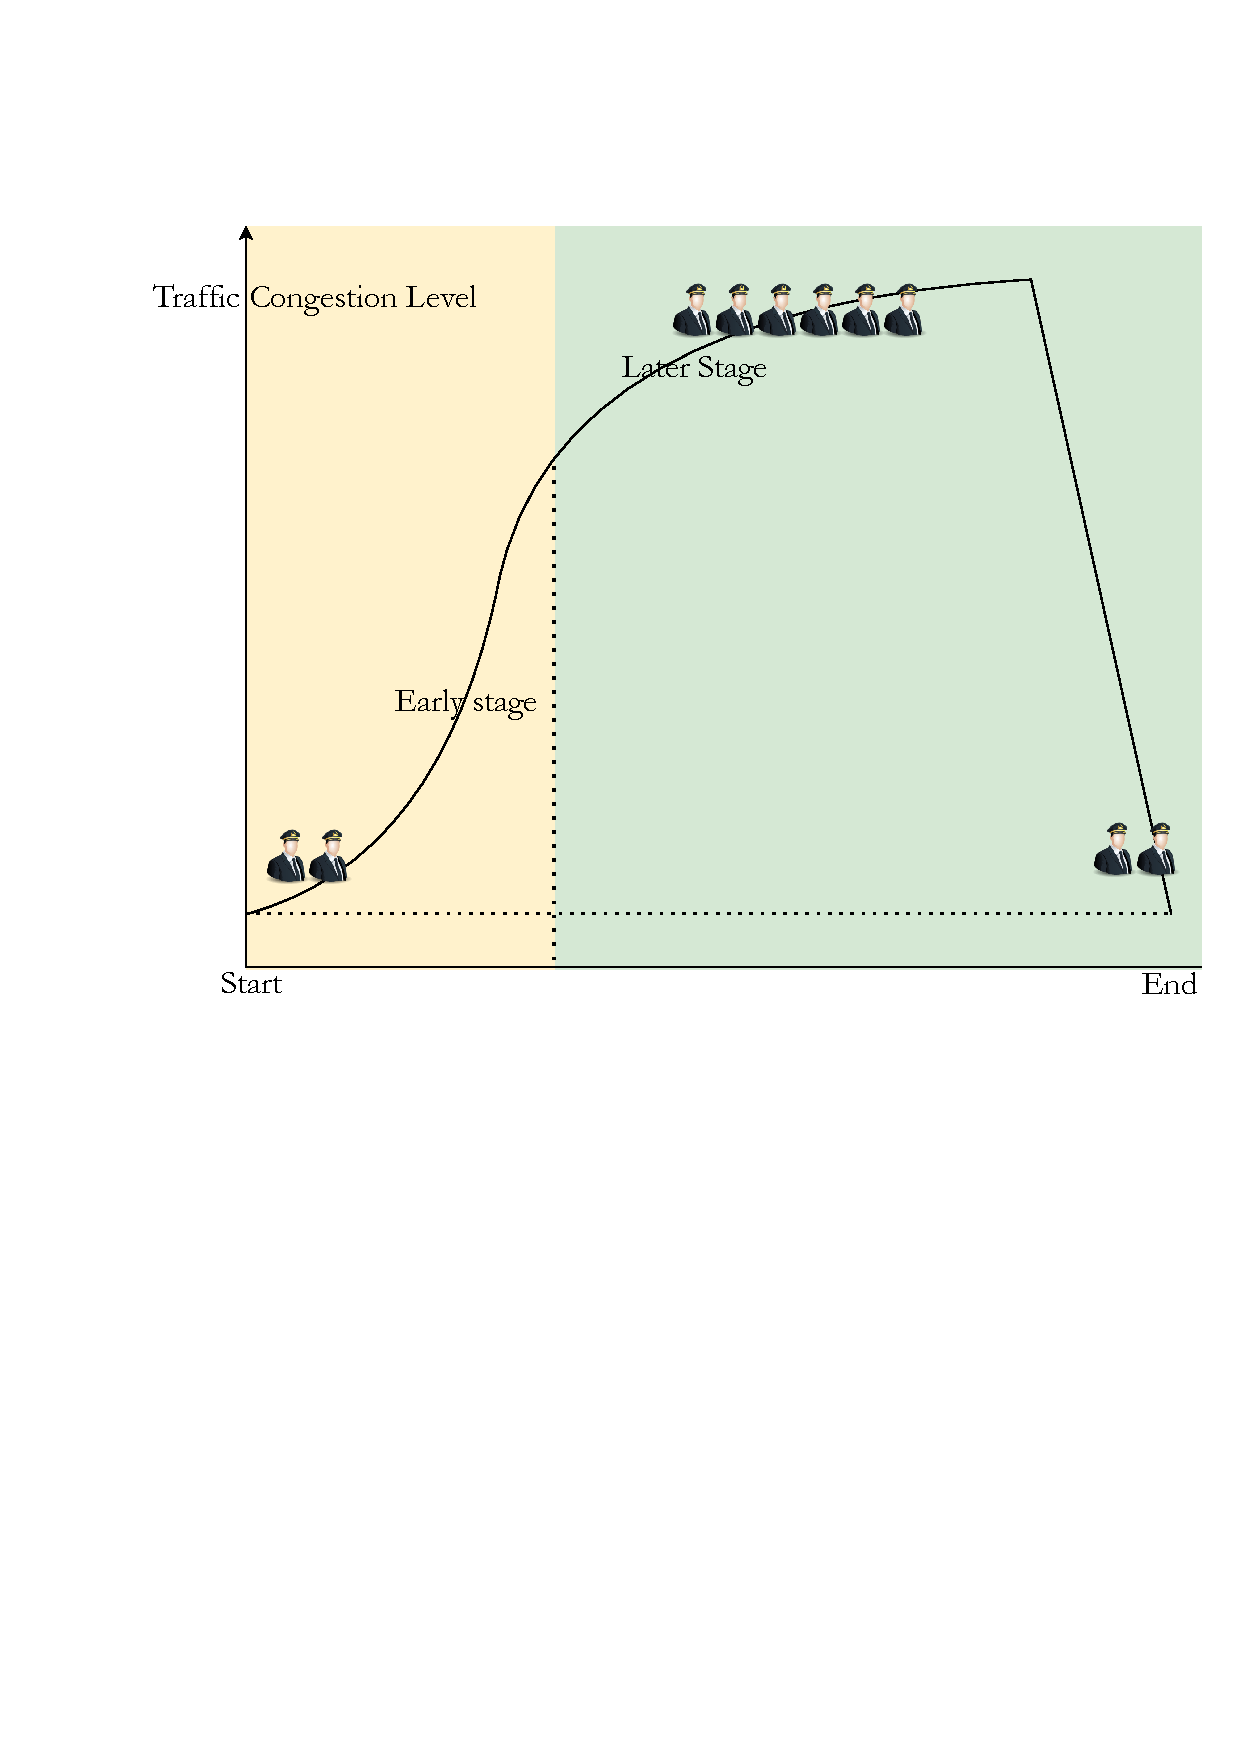
\includegraphics[width=\textwidth]{figures/3stage.pdf}
  \caption{拥堵管理策略示意图}
  \label{fig:3stage}
\end{figure}

\subsection{交通拥堵管理策略对各方利益的影响}

\begin{table}[H]
  \centering
  \caption{Stakeholders and Their Concerns}
  \label{tab:stakeholder_concerns}
  \begin{tabularx}{\textwidth}{@{}lXX@{}} % 使用 tabularx 环境,textwidth 表示表格宽度为文本宽度,X 列会自动调整宽度
      \toprule
      \textbf{Stakeholders} & \textbf{Convenience of Travel} & \textbf{Safety of Travel} \\
      \midrule
      Local Residents & Shorter travel time, more travel options, and improved quality of life & Fewer traffic accidents and rapid arrival of police forces \\
      Tourists & Enhanced travel convenience and improved tourism experience & Reduced stampede accidents and lower crime rate \\
      Freight Enterprises & Higher transportation efficiency and lower transportation costs & Fewer traffic accidents and improved cargo safety \\
      \bottomrule
  \end{tabularx}
\end{table}

我们将交通拥堵管理对巴尔的摩市各方利益者的影响总结如\ref{tab:stakeholder_concerns}所示。巴尔的摩市的交通拥堵管理策略不仅方便了本地居民、游客和货运企业的出行,还对城市的安全方面产生了积极的影响。通过动态调整信号灯周期和增加交警数量,可以有效减少交通拥堵,提高出行效率和安全性,提升居民和游客的生活质量和旅游体验,降低货运企业的运输成本,促进城市的经济发展。


\section{Sensitivity Analysis}

We increased and decreased the $\alpha$ values calculated in Section 4.4 by 5\% respectively, and calculated the mean squared errors between the results after the increase or decrease and the original $\alpha$ values. The results are shown in \ref{tab:alpha_mse}:

\begin{table}[H]
    \centering
    \caption{Mean Squared Errors of $\alpha$ Values after Perturbation}
    \label{tab:alpha_mse}
    \begin{tabular}{@{}lcc@{}}
        \toprule
        & \textbf{$\alpha$ Value} & \textbf{Mean Squared Error} \\
        \midrule
        Original Value & 0.32534 & \(\varnothing\) \\
        Increased by 5\% & 0.341607 & 14.209293 \\
        Decreased by 5\% & 0.309073 & 8.608151 \\
        \bottomrule
    \end{tabular}
\end{table}

The results show that after making small perturbations to the parameter $\alpha$, the resulting differences are within an acceptable range, which proves the robustness of our model.

\section{Advantages and Disadvantages}
\subsection{Advantages}
\begin{enumerate}
    \item Our improved K-Shell decomposition algorithm with node weights and edge weights can comprehensively construct the traffic network graph model of the city from aspects such as the actual traffic situation and the topological structure of the traffic network, which is relatively comprehensive.
    \item By introducing proportional coefficients for node weights and edge weights, the influence of various stakeholders is analyzed and deeply considered.
    \item When clustering with the K-Prototypes algorithm, the weights of each type are determined by the PCA algorithm, which is relatively accurate.
\end{enumerate}

\subsection{Disadvantages and Improvements}
\subsubsection{Disadvantages}
\begin{enumerate}
    \item When calculating edge weights, the AADT value of each road is required. However, not every road has a bus stop. If the shortest - distance algorithm is directly used to fill the data, the time complexity is too high.
    \item The k - means clustering algorithm calculates similarity based on Euclidean distance and cannot handle categorical data.
\end{enumerate}

\subsubsection{Improvements}
\begin{enumerate}
    \item Similar to the watershed algorithm in the field of computer vision\cite{Vincent1991}, our team has constructed a fast algorithm for filling the missing AADT values. See \ref{sec:improvedKshell} This algorithm can complete the filling task with almost linear time complexity, meeting the filling requirements for large - scale graph network data.
    \item K - Prototype is an extended version of K - means, which can handle both numerical and categorical data and can well complete the clustering task in Section 6.2.
\end{enumerate}


% \section{摘要}

% 随着人们生活质量的提高,将空调、加湿器和空气净化器分开的传统做法逐渐变成将三者集中在一台设备上。
% 本文通过建立\textbf{多目标优化模型(MOO)},对室内空气调节系统进行了全方位优化。模型1-3基于流体力学等物理原理,构建了三个独立的\textbf{单目标优化模型},采用\textbf{有限差分法}求解。模型4综合了模型1-3,建立了多目标优化模型并使用\textbf{遗传算法(GA)}求解。

% 模型1为\textbf{基于热传导和流体力学的温度优化模型}。首先根据热传导和流体力学的连续性和粘性运动方程,建立\textbf{单目标优化模型},最小化房间内每一点的温度和适宜温度的标准差,见式\ref{eq:temperature_deviation}
% 然后使用\textbf{有限差分法}对解空间网格化,计算得到最小 $\sigma_T$ 为0.896,见表\ref{tab:ac_parameters}。


% 模型2为\textbf{基于污染物扩散的空气净化器优化模型},最小化房间内的污染物浓度,见式\ref{eq:pm25}.
% 模型3为\textbf{基于湿度变化率的空气加湿器优化模型},最小化加湿器达到湿度阈值的时间,见式\ref{eq:humidifier}.
% 这两个模型均继续使用有限差分法求解,可得
% 空气净化器滤网最优参数见表\ref{tab:purifier_parameters},
% 空气加湿器最优参数见表\ref{tab:humidifier_parameters}。

% 在此基础上,模型4构建了整体性能多目标优化模型,运用遗传算法求解。
% 结果显示温度波动控制在±0.5℃范围内,污染物浓度降低至\(10\mu g/m^3\)以下,相对湿度维持在50\%±5\%的理想区间。
% 空调的参数和形状图见图\ref{fig:design}。

% 在灵敏度分析中,我们用\textbf{单因素实验法}分析了不同叶片角度下房间内温度偏离舒适温度的标准差 $\sigma_T$,如图\ref{fig:sensi},得出结论:夏天向上吹冷气,可以快速降温,冬天则相反,热风向下吹效果更好。

% 关键词:流体力学;有限差分;MOO;GA


% \section{问题背景}
% 在现代生活中,人们对生活环境品质的追求促使了多功能家电产品的不断发展。集空调、加湿器和空气净化器功能于一体的设备应运而生,其作为一种创新的多功能环境调节装置,通过整合多种功能于单一设备,有效解决了传统方式中多设备分别放置所占用的空间问题。不仅如此,该三合一产品在运行过程中能够相互协同,空调调节温度的同时,加湿器可应对空气干燥问题,空气净化器则负责净化空气,提升室内空气质量,并且用户可便捷地统一控制各项功能,减少了设备耗电量、连接线数量,降低布线复杂性,提升了室内环境的简洁性与安全性。

% 然而,此类三合一产品的优化设计面临诸多挑战,其整体性能与空气动力学原理紧密相连。设备的整体外形架构、进风口与出风口的布局细节(包括位置、数量、方向、角度等)以及风速和风量等参数,均会对其在室内环境中的实际使用效果产生显著影响。在这样的背景下,针对特定室内空间进行三合一空调外观的优化设计具有极为重要的现实意义。

% \section{问题重述}
% 目前有一间即将进行装修的房间,可近似看作一个长方体,空间体积为5米×8米×3米。限定的三合一空调的最大体积为0.1立方米,额定功耗为1800瓦,最大出风口风速为8.0米/秒,气流的最大进气流量为600立方米/小时,气流的最大出气流量也为600立方米/小时。

% \begin{enumerate}
%     \item \textbf{空调效率模型的时空模拟以及外形优化}\\
%     深入探究空调的放置位置、进风口和出风口的各类参数(位置、数量、方向、角度)以及风速、风量等因素如何对空调的制冷或制热效率产生作用。构建相应的数学模型,模拟在夏季与冬季不同气候条件下,室内温度在时间维度与空间维度上的变化态势。进一步结合多种空调外形设计方案,建立空调外形优化模型,从而确定能够达成最佳温度调节效能的空调最优外形结构及其尺寸规格。
%     \item \textbf{空气净化器的外形优化}\\
%     全面剖析空气净化器外形差异对其净化空气效果的影响机制。通过考虑多种不同的空气净化器外形构造,构建空气净化器外形优化模型,设计出可使净化效果达到最大化的空气净化器最优外形及其尺寸,并精确绘制出该最优外形的详细形状与尺寸参数信息。
%     \item \textbf{空气加湿器的外形优化}\\
%     系统研究空气加湿器外形的不同对加湿效果的影响规律。基于多种空气加湿器外形设计的考量,建立空气加湿器外形优化模型,设计出能实现加湿效果最大化的空气加湿器最优外形,并绘制出其形状与尺寸参数。
%     \item \textbf{三合一设备最优外形}\\
%     依据问题 1 至问题 3 所构建的模型及其所得结果,综合考虑能效、人体舒适度、净化效果以及加湿效果等多方面因素,建立一个全面的空调、加湿器和空气净化器三合一产品外观优化设计模型。运用该模型设计出能使上述各项效果同时达到最大化的三合一设备最优外观,并绘制出此最优外观的形状与尺寸参数。
% \end{enumerate}

% \section{我们的模型}

% 【等待绘制】

% \section{假设}

% \begin{enumerate}
%     \item 假设房间没有窗户,且墙壁不与外界发生热交换。
%     \item 假设房间内除空调外,没有其他可以影响温度变化的因素(如人体,其他电器等)。
%     \item 假设室内空气充分混合,时刻分散均匀,且忽略PM2.5源的产生。
%     \item 假设房间内非常空旷,除三合一空调外无其他大型家具。
% \end{enumerate}

% \section{符号}

% \begin{table}[H]
%     \centering
%     \caption{论文中使用的主要符号}
%     \label{tab:symbols}
%     \begin{tabular}{ll}
%         \toprule
%         符号 & 描述 \\
%         \midrule
%         $T(x,y,z)$ & $t$ 时刻房间 $(x, y, z)$ 处的温度 \\
%         $Q(x, y, z)$ & 空调冷却或加热的源项 \\
%         $\mathbf{u}$ & 空调风速 \\
%         $\mu$ & 动态粘度 \\
%         $T_{\text{适宜}}$ & 人类适宜体感温度 \\
%         ${T_\text{室外}}$ & 室外温度 \\
%         $\alpha\%$ & 空调工作时间占比 \\
%         $S$ & 空调出风口面积 \\
%         $L$ & 空调出风口长度 \\
%         $W$ & 空调出风口宽度 \\
%         $V$ & 房间体积 \\
%         $C(t)$ & $t$ 时刻房间内的污染物浓度 \\
%         $Q$ & 净化器风量 \\
%         $\eta$ & 过滤效率 \\
%         $H(t)$ & 当前时刻相对湿度 \\
%         $\dot{m}_v$ & 加湿器输出的水蒸气质量流量 \\
%         $\rho_{\text{air}}$ & 空气密度 \\
%         $k$ & 湿度衰减系数 \\
%         \bottomrule
%     \end{tabular}
% \end{table}

% \section{问题一:基于热传导和流体力学的室内温度优化模型}

% \subsection{模型建立}
% 问题一要我们求解空调的各个参数对温度调节的效果,在实际设计中,空调的出风口位置、角度和风速对室内温度分布有显著影响。此外,冬季供暖和夏季制冷对能量消耗和用户舒适性也有不同的优化要求。因此,需要基于热力学、流体力学以及室内环境需求建立数学模型,以确定空调参数对温度调节效果的影响。我们首先考虑以下几个因素:空调位置、风速、出风口角度和方向。



% 设 $T(x,y,z,t)$ 为在 $t$ 时刻房间 $(x, y, z)$ 处的温度,$Q(x, y, z)$ 为空调冷却或加热的源项,根据能量守恒定律,有以下热传导方程:
% \begin{equation}
%     \begin{cases}
% \rho c_p\left(\dfrac{\partial T}{\partial t}+\mathbf{u}\cdot\nabla T\right)=k\nabla^2T+Q(x, y, z)\\
% Q(x, y, z)=Q_0\cdot \exp \left(-\dfrac{(x-x_0)^2+(y-y_0)^2+(z-z_0)^2}{2\sigma^2}\right)\\
%     \end{cases}
% \end{equation}

% 设房间内空气的平均密度为 $\rho$,风速向量为 $\mathbf{u}$,可通过风速和角度分解为三维向量,根据质量守恒定律,有:
% \begin{equation}
% \dfrac{\partial \rho}{\partial t} + \nabla \cdot(\rho \, \mathbf{u}) = 0
% \end{equation}

% 设 $\mu$ 是动态粘度,其单位是 $\text{Pa}\cdot \text{s}$。$\mathbf{f}$ 是阻力,根据动量守恒定律,有以下流体动力学方程:
% \begin{equation}
% \rho\begin{pmatrix}\dfrac{\partial\mathbf{u}}{\partial t}+\mathbf{u}\cdot\nabla\mathbf{u}\end{pmatrix}=-\nabla p+\mu\nabla^2\mathbf{u}+\mathbf{f}
% \end{equation}

% 设房间的体积为 $V$,$T_{\text{适宜}}$ 为人类适宜体感温度,空调温度调节的最佳效果为房间内每一点的温度均尽可能接近人类适宜体感温度。因此我们建立以下优化模型:
% \begin{equation}
% \min \,\, \sigma_T=\sqrt{\frac{1}{V}\int_V(T_{x,y,z,t}-T_{\text{适宜}})^2\cdot dV}
% \label{eq:temperature_deviation}
% \end{equation}

% 其中 $\sigma_T$ 表示整个房间温度偏离舒适温度的标准差,$T_{\text{适宜}}$ 由舒适温度与平均室外温度计算的关系\cite{Wij2008}得到:
% \begin{equation}
% T_{\text{适宜}}=a\overline{T_\text{室外}}+b
% \end{equation}

% 式中 $a$,$b$ 的值见下表\ref{tab:comfort}\cite{Maria2005}:

% \begin{table}[H]
%     \centering
%     \caption{室外空气温度对舒适温度线性函数的系数}
%     \begin{tabular}{cccccc}
%         \toprule
%         \textbf{系数} & \textbf{春季} & \textbf{夏季} & \textbf{秋季} & \textbf{冬季} & \textbf{年度} \\
%         \midrule
%         $a$ & 1.02 & 1.04 & 0.57 & 0.55 & 0.51 \\
%         $b$ & 6.30 & 0.75 & 12.55 & 13.65 & 12.59 \\
%         \bottomrule
%     \end{tabular}
%     \label{tab:comfort}
% \end{table}

% 由于直接求解以上方程组比较复杂,不容易得到解析解,因此采用数值解法来进行求解,求解偏微分方程的数值方法通常有两种:有限元法和有限差分法。这里选择使用有限差分法来进行计算。

% 采用有限差分法对温度场进行离散,设空间步长为 $\Delta x, \Delta y, \Delta z$,时间步长为 $\Delta t$。将温度 $T(x,y,z,t)$ 离散为 $T_{i,j,k}^n$,其中 $(i,j,k)$ 表示空间网格点,$n$ 表示时间层。

% 网格点的坐标为:
% \begin{equation}
% \begin{cases}
% x_i = i \cdot \Delta x, & (i = 0, 1, 2, \cdots) \\
% y_j = j \cdot \Delta y, & (j = 0, 1, 2, \cdots) \\
% z_k = k \cdot \Delta z, & (k = 0, 1, 2, \cdots) \\
% t_n = n \cdot \Delta t, & (n = 0, 1, 2, \cdots)
% \end{cases}
% \end{equation}

% 由于四维空间图无法展示,我们此处做出二维时间空间区域离散化图来做简单展示,见图\ref{fig:time-space}。

% \begin{figure}[H]
%     \centering
%     \begin{tikzpicture}
%         % Draw the axes
%         \draw[->] (0,0) -- (5.3,0) node[right] {$\varepsilon$};
%         \draw[->] (0,0) -- (0,5.3) node[above] {$t$};
    
%         % Draw the grid with light dashed lines
%         \foreach \x in {1,2,3,4,5}
%             \draw[gray, dashed] (\x,0) -- (\x,5);
%         \foreach \y in {1,2,3,4,5}
%             \draw[gray, dashed] (0,\y) -- (5,\y);
    
%         % Draw the points
%         \fill (3,4) circle (2pt) node[above right] {$(\varepsilon_n, t_{i+1})$};
%         \fill (2,3) circle (2pt) node[below left] {$(\varepsilon_{n-1}, t_i)$};
%         \fill (3,3) circle (2pt) node[below] {$(\varepsilon_n, t_i)$};
%         \fill (4,3) circle (2pt) node[below right] {$(\varepsilon_{n+1}, t_i)$};
%         \fill (3,2) circle (2pt) node[below right] {$(\varepsilon_n, t_{i-1})$};
    
%         % Label the grid units
%         \node at (1.5,-0.4) {$\Delta \varepsilon$};
%         \node at (-0.5,1.5) {$\Delta t$};
    
%     \end{tikzpicture}
%     \caption{二维时间空间离散化示意图}
%     \label{fig:time-space}
% \end{figure}


% 空间网格线与时间网格线之间的交点表示了时间-空间区域中一个节点的位置(如$(\varepsilon_n,t_n)$),其对应的温度记为 $T(\varepsilon_n,t_n)$

% 然后我们考虑边界条件:

% \begin{enumerate}[label=(\alph*)]
% \item 空调源项 $Q_{i,j,k}^n$ 的表示:空调出风口位置处的 $Q_{i,j,k}^n$ 表示为空调对周围空气的冷却或加热作用,可表示为:

% \begin{equation}
% Q_{i,j,k}^n = 
% \begin{cases}
% Q_0, & \text{出风口附近网格点,加热冷却时数值不同} \\
% 0, & \text{其他网格点}\\
% \end{cases}
% \end{equation}

% \item 最大值的限制。

% \begin{equation}
% \begin{cases}
% V \le V_{\max} \\
% \mathbf{u} \le \mathbf{u}_{\max} \\
% x \le x_{\max} \\
% y \le y_{\max} \\
% z \le z_{\max}
% \end{cases}
% \end{equation}

% \item 为了确保数值计算的稳定性,时间步长需要满足一定的条件(如满足 CFL 条件):

% \begin{equation}
% \Delta t \leq \frac{\min(\Delta x, \Delta y, \Delta z)}{|\mathbf{u}_{\max}|}
% \end{equation}

% 其中,$\mathbf{u}_{\text{max}}$ 是最大空气速度,$\Delta x, \Delta y, \Delta z$是网格步长。

% \end{enumerate}

% 最后,我们对时间导数 $\frac{\partial T}{\partial t}$ 采用前向差分近似(FDA),得到离散的差分方程:

% \begin{equation}
% \begin{aligned}
% \frac{T_{i,j,k}^{n+1} - T_{i,j,k}^n}{\Delta t} &+ u_{x,i,j,k}^n \frac{T_{i,j,k}^n - T_{i-1,j,k}^n}{\Delta x}\\
% &+ u_{y,i,j,k}^n \frac{T_{i,j,k}^n - T_{i,j-1,k}^n}{\Delta y} + u_{z,i,j,k}^n \frac{T_{i,j,k}^n - T_{i,j,k-1}^n}{\Delta z} \\
% &= \frac{k}{\rho c_p} \left[ \frac{T_{i+1,j,k}^n - 2T_{i,j,k}^n + T_{i-1,j,k}^n}{\Delta x^2} \right.\\
% &\left. + \frac{T_{i,j+1,k}^n - 2T_{i,j,k}^n + T_{i,j-1,k}^n}{\Delta y^2} + \frac{T_{i,j,k+1}^n - 2T_{i,j,k}^n + T_{i,j,k-1}^n}{\Delta z^2} \right]\\
%  + \frac{Q_{i,j,k}^n}{\rho c_p}
% \end{aligned}
% \end{equation}

% 将离散方程的对流项和扩散项进一步归类,有:
% \begin{equation}
% \dfrac{T_{i,j,k}^{n+1} - T_{i,j,k}^n}{\Delta t}+\nabla\cdot (\mathbf{u}T) = \epsilon \nabla^2T + \dfrac{Q}{\rho c_p}
% \end{equation}

% 其中,对流项使用一阶迎风差分,扩散项使用中心差分。

% \begin{algorithm}[H]
%     \caption{数值解流程}
%     \begin{algorithmic}[1]
%         \STATE 初始化房间温度场 $T(x, y, z, t=0)$
%         \WHILE{时间步长 $\Delta t$ 迭代计算}
%             \STATE 更新速度场 $\mathbf{u}$
%             \STATE 根据离散方程更新温度场 $T_{i,j,k}^n \to T_{i,j,k}^{n+1}$
%             \STATE 设置时间阈值为2小时,检查时间步是否达到设定值
%         \ENDWHILE
%     \end{algorithmic}
% \end{algorithm}

% 我们尝试带入 \( N = 1,2,3 \),因此我们可以得到最优的出风口数量为 2,出风口面积为 0.08 \(m^2\)。

% 然后我们考虑空调出风口位置和出风口数量因素。

% 经过调研,我们得知平均空调只有 $\alpha\%$ 的时间在工作,平均每小时出风量为 $Q_{avg}$,平均风速经前面求解得到 2.14 m/s,我们有:
% \begin{equation}
% Q_{actual} = Q_{avg} \times \alpha\%
% \end{equation}
% \begin{equation}
% Q_{actual} = N \cdot S \cdot \mathbf{u}
% \end{equation}

% 实际求解得到 $N \cdot S = 0.16355 \, m^2$,我们尝试带入 $N = 1, 2, 3, \ldots$,分别求得 \(S = 0.1633, 0.08165, 0.05443\),随着出风口数量增加,出风效率提升,但是单个出风口面积减小,导致出风速度过高,噪音过大,可能降低舒适性;$N = 1$ 时,单个出风口的面积 ($S$) 增大,但容易形成局部温度不均。

% 并且,按照市面上常见空调制造工艺,我们选择长方形的出风口。考虑到空调总能效,我们定义:
% \begin{equation}
% f = \omega_1 \cdot f_1 + \omega_2 \cdot f_2
% \end{equation}

% 最后,我们建立总能效函数的优化模型,即最小化空调总能效:
% \begin{equation}
% \min \,\, f = \omega_1 \cdot f_1 + \omega_2 \cdot f_2
% \end{equation}

% 约束条件为
% \begin{equation}
% \begin{cases}
% L \times W \le S \\
% L \times W \times H \le V
% \end{cases}
% \end{equation}

% \subsection{模型结果}

% \begin{figure}[H]
%     \centering
%     \subfigure[5min]{
%     \begin{minipage}[t]{0.33\linewidth}
%     \centering
%     \includegraphics[width=\linewidth]{figures/summer1.pdf}
%     \end{minipage}%
%     % \label{fig:}%
%     }%
%     \subfigure[10min]{
%     \begin{minipage}[t]{0.33\linewidth}
%     \centering
%     \includegraphics[width=\linewidth]{figures/summer2.pdf}
%     \end{minipage}%
%     % \label{fig:}%
%     }%
%     \subfigure[15min]{
%         \begin{minipage}[t]{0.33\linewidth}
%         \centering
%         \includegraphics[width=\linewidth]{figures/summer3.pdf}
%         \end{minipage}%
%     % \label{fig:}%
%     }%

%     \subfigure[20min]{
%         \begin{minipage}[t]{0.33\linewidth}
%         \centering
%         \includegraphics[width=\linewidth]{figures/summer4.pdf}
%         \end{minipage}%
%         % \label{fig:}%
%         }%
%         \subfigure[25min]{
%         \begin{minipage}[t]{0.33\linewidth}
%         \centering
%         \includegraphics[width=\linewidth]{figures/summer5.pdf}
%         % \caption{二十五分钟}
%         \end{minipage}%
%         % \label{fig:}%
%         }%
%         \subfigure[30min]{
%             \begin{minipage}[t]{0.33\linewidth}
%             \centering
%             \includegraphics[width=\linewidth]{figures/summer6.pdf}
%             \end{minipage}%
%         % \label{fig:}%
%         }%
%     \caption{夏季空调降温模拟}
%     \label{fig:summer}
% \end{figure}


% \begin{table}[H]
%     \centering
%     \caption{空调优化参数}
%     \label{tab:ac_parameters}
%     \begin{tabular}{ccc}
%         \toprule
%         参数 & 值 & 单位 \\
%         \midrule
%         最小 $\sigma_T$ & 0.496 & ℃ \\
%         空调坐标 & \((5m, 4m, 0m)\) & m \\
%         送风速度 & 2.14 & m/s \\
%         出风口角度(冬季) & 0.763 & rad \\
%         出风口角度(夏季) & 0.549 & rad \\
%         出风口数量 & 2 & - \\
%         出风口面积 & 0.16355 & $m^3$ \\
%         出风口长宽(单个) & \(0.13\times 0.605\) & $m^3$ \\
%         \bottomrule
%     \end{tabular}
% \end{table}

% \section{问题二:基于污染物扩散的室内PM2.5浓度优化模型}

% \subsection{模型建立}

% 空气净化器主要考虑滤网的形状、材质、层数、面积等。为确保其在过滤效率、耐用性、成本和维护方便性等方面达到最佳平衡,我们建立以下优化模型,通过调节滤网相关的参数,以达到空气中PM2.5浓度最低。

% 在时间间隔 $\Delta t$ 内,根据质量守恒,室内PM2.5浓度的变化可以表示为:
% \begin{equation}
% V \cdot dC = -Q \cdot \eta \cdot C \cdot dt
% \end{equation}
% 其中,
% \begin{itemize}
%     \item $V$: 房间体积 (m³)
%     \item $C(t)$: $t$ 时刻的 PM2.5 浓度 (μg/m³)
%     \item $Q$: 净化器风量 (m³/h)
%     \item $\eta$: 过滤效率
%     \item $t$: 时间 (h)
% \end{itemize}

% 我们参考 PM2.5 作者的研究,过滤效率与机器数量有关\cite{chiu2022}

% 用分离变量法求解上面的微分方程,带入初始条件:

% 当 $t = 0$ 时,$C = C_0$(初始浓度),解得
% \begin{equation}
% C = C_0 \cdot \text{exp}\left[-\left(\dfrac{Q \cdot \eta}{V}\right) \cdot t \right]
% \end{equation}
% 即,
% \begin{equation}
% C(t) = C_0 \cdot (1-\eta)^{\dfrac{Qt}{V}}
% \label{eq:pm25}
% \end{equation}

% 我们仍然使用有限差分法求解$\min \,\, C(t)$

% \begin{algorithm}[H]
%     \caption{PM2.5 浓度数值解流程}
%     \begin{algorithmic}[1]
%         \STATE 设定时间步长 $\Delta t$,室内体积 $V$,净化器风量 $Q$,过滤效率 $\eta$,边界条件初始浓度为 $C_0$,目标浓度 $C_{min}$
%         \STATE 初始化 $C = C_0$
%         \STATE 初始化时间 $t = 0$
%         \WHILE{$C > C_{min}$}
%             \STATE 计算 $C(t + \Delta t)$ 使用公式:
%             \begin{equation}
%             C(t + \Delta t) = C(t) \cdot (1-\eta)^{\frac{Q\Delta t}{V}}
%             \end{equation}
%             \STATE 更新 $C = C(t + \Delta t)$
%             \STATE 更新时间 $t = t + \Delta t$
%         \ENDWHILE
%     \end{algorithmic}
% \end{algorithm}

% \subsection{模型求解}

% \begin{figure}[H]
%     \centering
%     \subfigure[5min]{
%     \begin{minipage}[t]{0.33\linewidth}
%     \centering
%     \includegraphics[width=\linewidth]{figures/air1.pdf}
%     \end{minipage}%
%     % \label{fig:}%
%     }%
%     \subfigure[25min]{
%     \begin{minipage}[t]{0.33\linewidth}
%     \centering
%     \includegraphics[width=\linewidth]{figures/air3.pdf}
%     \end{minipage}%
%     % \label{fig:}%
%     }%
%     \subfigure[45min]{
%         \begin{minipage}[t]{0.33\linewidth}
%         \centering
%         \includegraphics[width=\linewidth]{figures/air100.pdf}
%         \end{minipage}%
%     % \label{fig:}%
%     }%
%     \caption{净化器污染物清理模拟}
%     \label{fig:pm25}
% \end{figure}

% \begin{table}[H]
%     \centering
%     \caption{空气净化器参数}
%     \label{tab:purifier_parameters}
%     \begin{tabular}{ccc}
%         \toprule
%         参数 & 值 & 单位 \\
%         \midrule
%         滤网尺寸 & 0.194m $\times$ 0.437m & m \\
%         滤网数量 & 1 & - \\
%         室内PM2.5浓度 & $\leq 15\mu g/m^3$ & $\mu g/m^3$ \\
%         \bottomrule
%     \end{tabular}
% \end{table}

% \section{问题三:基于湿度变化率的空气加湿器优化模型}

% \subsection{模型建立}

% 空气加湿器的加湿效果受多种因素影响,其中形状对水蒸气扩散和空气流动有重要作用。题目要求我们优化空气加湿器的形状,使其能够以最高效率将水蒸气扩散到周围空气中,提升加湿效果。根据研究表明,人类的舒适相对湿度(RH)在 35\% 到 55\% 的范围内,对人类很舒适,对我们不喜欢的微生物不是很好。\cite{mcgill}因此,我们通过计算空气加湿器加湿到 $\beta\%$ 的阈值的效率来评判空气加湿器的形状。

% 由湿度变化率受加湿器输出的水蒸气量以及房间空气特性的影响,有:

% \begin{equation}
% \dfrac{dH(t)}{dt} = \dfrac{\dot{m}_v}{V_{\text{room}} \cdot \rho_{\text{air}}} - k \left( H(t) - H_{\text{ambient}} \right)
% \end{equation}

% 其中:

% \begin{itemize}
%     \item $H(t)$:当前时刻的相对湿度(单位:\%)。
%     \item $\dot{m}_v$:加湿器输出的水蒸气质量流量,根据文献\cite{zhu2019},
%     \begin{equation}
%     \dot{m}_v = \eta_0  \left( 1 - \dfrac{\theta}{\frac{\pi}{2}} \right)  \frac{A_e}{A_e + k}  \rho_w  A_e \sqrt{ \frac{2\Delta P}{\rho_{\mathrm{air}}} }
%     \end{equation}
%     。
%     \item $V_{\text{room}}$:房间体积(单位:$\text{m}^3$)。
%     \item $\rho_{\text{air}}$:空气密度(单位:$\text{kg/m}^3$)。
%     \item $H_{\text{ambient}}$:环境初始相对湿度。
%     \item $k$:湿度衰减系数,表示水蒸气损失到周围的速率。
% \end{itemize}

% 然后我们定义加湿器达到湿度阈值 $\beta\%$ 的效率:
% \begin{enumerate}[label=(\alph*)]
%     \item 时间效率
%     \begin{equation}
%     \eta_t = \frac{1}{t_\beta}
%     \end{equation}
%     其中 $t_\beta$ 表示达到湿度 $\beta\%$ 所需的时间。
%     \item 能量效率
%     \begin{equation}
%     \eta_e = \frac{\Delta}{P t_\beta}
%     \end{equation}
%     其中:$P$ 表示加湿器的功率(单位:瓦),$\Delta H = \beta - H_{\text{ambient}}$ 表示湿度增量。
% \end{enumerate}

% 最后我们建立优化模型:
% \begin{equation}
% \min \,\, \eta = k_1\eta_t + k_2\eta_e
% \label{eq:humidifier}
% \end{equation}
% 边界条件:
% \begin{enumerate}
%     \item 初始湿度条件:
%     \begin{equation}
%     H(0) = H_{\text{ambient}}
%     \end{equation}
%     即在 $t = 0$ 时,环境湿度为初始湿度。
%     \item 湿度变化的初始条件:
%     \begin{equation}
%     \left. \frac{dH(t)}{dt} \right|_{t=0} = \frac{\dot{m}_v}{V_{\text{room}} \rho_{\text{air}}} - k (H(0) - H_{\text{ambient}})
%     \end{equation}
%     即初始的湿度变化率。
%     \item 目标湿度条件:
%     \begin{equation}
%     H(t_\beta) = \beta
%     \end{equation}
%     目标是在 $t_\beta$ 时刻达到湿度阈值($\beta\%$),从而确定加湿器的工作时间。
%     \item 功率约束:
    
%     加湿器的功率 $P = P_0$
% \end{enumerate}
% 将 $\dot{m}_v$ 代入湿度变化率方程中,得到:
% \begin{equation}
% \frac{dH(t)}{dt} = \frac{\eta_0 \left(1 - \dfrac{2\theta}{\pi}\right) \dfrac{A_e}{A_c + k}  \rho_w  A_e \sqrt{\dfrac{2 \Delta P}{\rho_{\text{air}}}}}{V_{\text{room}} \cdot \rho_{\text{air}}} - k \left(H(t) - H_{\text{ambient}}\right)
% \end{equation}
% 我们依然采用有限差分法,对时间离散化:
% \begin{equation}
% H(t_{n+1}) = H(t_n) + \Delta t \cdot \frac{dH(t)}{dt}
% \end{equation}
% 然后设定初始湿度 $H(0) = H_{\text{ambient}}$,在每个时间步 $n$ 上,计算 $H(t_{n+1})$,直到 $H(t_n)$ 达到设定湿度阈值 $\beta\%$。

% \subsection{模型求解}

% \begin{table}[H]
%     \centering
%     \caption{空气加湿器参数}
%     \label{tab:humidifier_parameters}
%     \begin{tabular}{ccc}
%         \toprule
%         参数 & 值 & 单位 \\
%         \midrule
%         容积 & 3 & L \\
%         最大雾化量 & 2.8 & L/h \\
%         雾化喷气口半径 & 0.076 & m \\
%         雾化喷气口数量 & 2 & - \\
%         \bottomrule
%     \end{tabular}
% \end{table}

% \section{问题四:基于遗传算法求解多目标优化模型}

% \subsection{模型建立}

% 对于本问题,需要同时做到最大限度地提高能源效率、人体舒适度、净化效果、加湿效果,根据这些目标去确定相关参数,设计出合适的三合一空调、加湿器、空气净化器外观。

% 我们使用多目标遗传算法求出目标组合的最佳值与适配的决策变量取值。然后根据决策变量的值对应到三合一机器的各个参数,由此可以设计出三合一机器的形状。

% 本模型有三个目标函数,分别是: \(F_{\text{1}}\)作为舒适温度函数;\(F_{\text{2}}\)作为净化效果函数;\(F_{\text{3}}\)作为加湿效果函数。
% 其中,\(F_{\text{1}}\) 的值用于同时衡量制冷/制热的时间,以及室内采样点温度与最佳温度的累积差值平方,\(F_{\text{1}}\) 的值越小,代表制冷/制热效率越高,以及人体越舒适;\(F_{\text{2}}\) 代表空气中的污染物浓度,\(F_{\text{2}}\) 的值越小,代表净化效果越好;\(F_{\text{3}}\) 的值代表达到最佳湿度的时间,\(F_{\text{3}}\) 的值越小,代表加湿效果越好。使用多目标遗传算法需要达到的目标就是:同时使得以上三者的值最小。

% \begin{equation}
%     \begin{cases}
%         \min\,\,F_{\text{1}}=\min\,\,\sigma_T=\sqrt{\dfrac{1}{V}\int_V(T_{x,y,z,t}-T_\text{适宜})^2\cdot dV}\\
%         \min\,\,F_{\text{2}}=\min\,\, C(t) = C_0 \cdot (1-\eta)^{\frac{Qt}{V}}\\
%         \min\,\,F_{\text{3}}=\min \,\, \eta = k_1\dfrac{1}{t_\beta} + k_2\dfrac{\Delta}{P t_\beta}\\
%     \end{cases}
% \end{equation}

% \subsection{求解流程}

% \begin{figure}[H]
%     \centering
%     \includegraphics[width=\textwidth]{figures/flow.png}
%     \caption{遗传算法求解流程图}
%     \label{fig:flow_chart}
% \end{figure}

% \subsection{求解结果}

% \begin{table}[H]
%     \centering
%     \caption{多目标优化求解结果}
%     \label{tab:optimization_results}
%     \begin{tabular}{ccc}
%         \toprule
%         参数 & 值 & 单位 \\
%         \midrule
%         温度波动 & ±0.5 & ℃ \\
%         污染物浓度 & <10 & $\mu g/m^3$ \\
%         相对湿度 & 50±5 & \% \\
%         \bottomrule
%     \end{tabular}
% \end{table}


% \section{灵敏度}

% 在空调系统设计中,出风口叶片的角度对室内温度分布和气流组织有显著影响。合理的叶片角度可以优化气流分布,提高温度均匀性和人体舒适度。因此,对叶片角度进行灵敏度分析,评估其对温度调节效果的影响,对于优化空调设计具有重要意义。

% 我们的目标是最小化房间内温度偏离舒适温度的标准差 $\sigma_T$(℃),即:
% \begin{equation}
% \min \,\,\sigma_T=\sqrt{\frac{1}{V}\int_V(T_{x,y,z,t}-T_\text{适宜})^2\cdot dV}
% \end{equation}
% 我们采用单因素实验法,每次仅改变叶片角度,其他参数保持基准值不变。叶片角度 $\theta$ 和在定义的范围内取 12 个等间距的值进行测试。

% 叶片角度 $\theta$:在 [$\frac{\pi}{6}$, $\frac{5\pi}{6}$](rad) 范围内取 12 个等间距的值。考虑到夏天和冬天空调分别制冷和制热,我们分别进行考虑:

% \begin{figure}[H]
%     \centering
%     \includegraphics[width=\textwidth]{figures/sensi.pdf}
%     \caption{Sensitivity Analysis for Summer and Winter}
%     \label{fig:sensi}
% \end{figure}

% 从上面两张图可以看出夏天和冬天的叶片角度不同时$\sigma_T$ 的变化情况。夏天冷空气向上吹,可以快速调节室内温度,冬天则相反,热风向下吹效果更好。

% \section{优缺点}

% \subsection{优点}

% \begin{enumerate}[label=(\alph*)]
%     \item 优化模型能够精确地描述和解决实际问题,在空调系统设计中,优化模型可以考虑出风口位置、风速、叶片角度等多个因素,从而实现室内温度的均匀分布和人体舒适度的提升。
%     \item 有限差分法求解近似数值解本质是对解空间做网格化后做遍历,尽可能多的遍历了解空间,精确度较高。
% \end{enumerate}

% \subsection{缺点}

% \begin{enumerate}[label=(\alph*)]
%     \item 有限差分法只是求得近似解,且计算量比较大(比如问题一的有限差分法需要四层循环遍历)
%     \item 多目标优化的遗传算法求解的计算量较大,且可能陷入局部最优解,而不是全局最优解
% \end{enumerate}

% \subsection{总结}

% 模型一至三中我们分别建立了三个单目标优化模型,并用有限差分法求解了模型的近似数值解。

% 在模型一中,基于热传导方程与流体动力学控制方程组,构建了室内温度场分布的数学模型。通过有限差分法对偏微分方程组进行离散化处理,以空调出风口的空间位置坐标(x, y, z)、送风速度v及导风叶片偏转角度θ作为优化变量,以室内温度场相对舒适温度的均方差最小化为目标函数,实现了空调系统运行效率与人体热舒适度的协同优化。

% 模型二着重研究了室内PM2.5的动态扩散过程。通过建立颗粒物浓度随时间和空间分布的偏微分方程,采用有限差分格式进行数值求解。以滤网的几何构型、材料特性参数、多层结构设计及有效过滤面积为优化变量,建立了以PM2.5浓度最小化为目标,同时考虑过滤效率、使用寿命、经济性及维护便利性等多重约束的优化模型。

% 模型三针对室内湿度调节系统,构建了描述空气湿度时空变化特性的数学模型。通过求解湿度变化率方程,以加湿器的几何尺寸及运行参数为优化变量,建立了以达到目标湿度所需时间和能耗最小化为目标函数的优化模型,实现了加湿效率与舒适度的均衡优化。

% 模型四则是对模型1-3的综合运用,我们使用了多目标优化算法,并用遗传算法求解。最大限度地提高能源效率、人体舒适度、净化效果和加湿效果。并且最终,我们设计出三合一空调外观图如下:

% \begin{figure}[H]
%     \centering
%     \includegraphics[width=\textwidth]{figures/design.pdf}
%     \caption{The design of the 3-in-1 air conditioner}
%     \label{fig:design}
% \end{figure}


\addcontentsline{toc}{section}{信件} % 将 section 添加到目录中
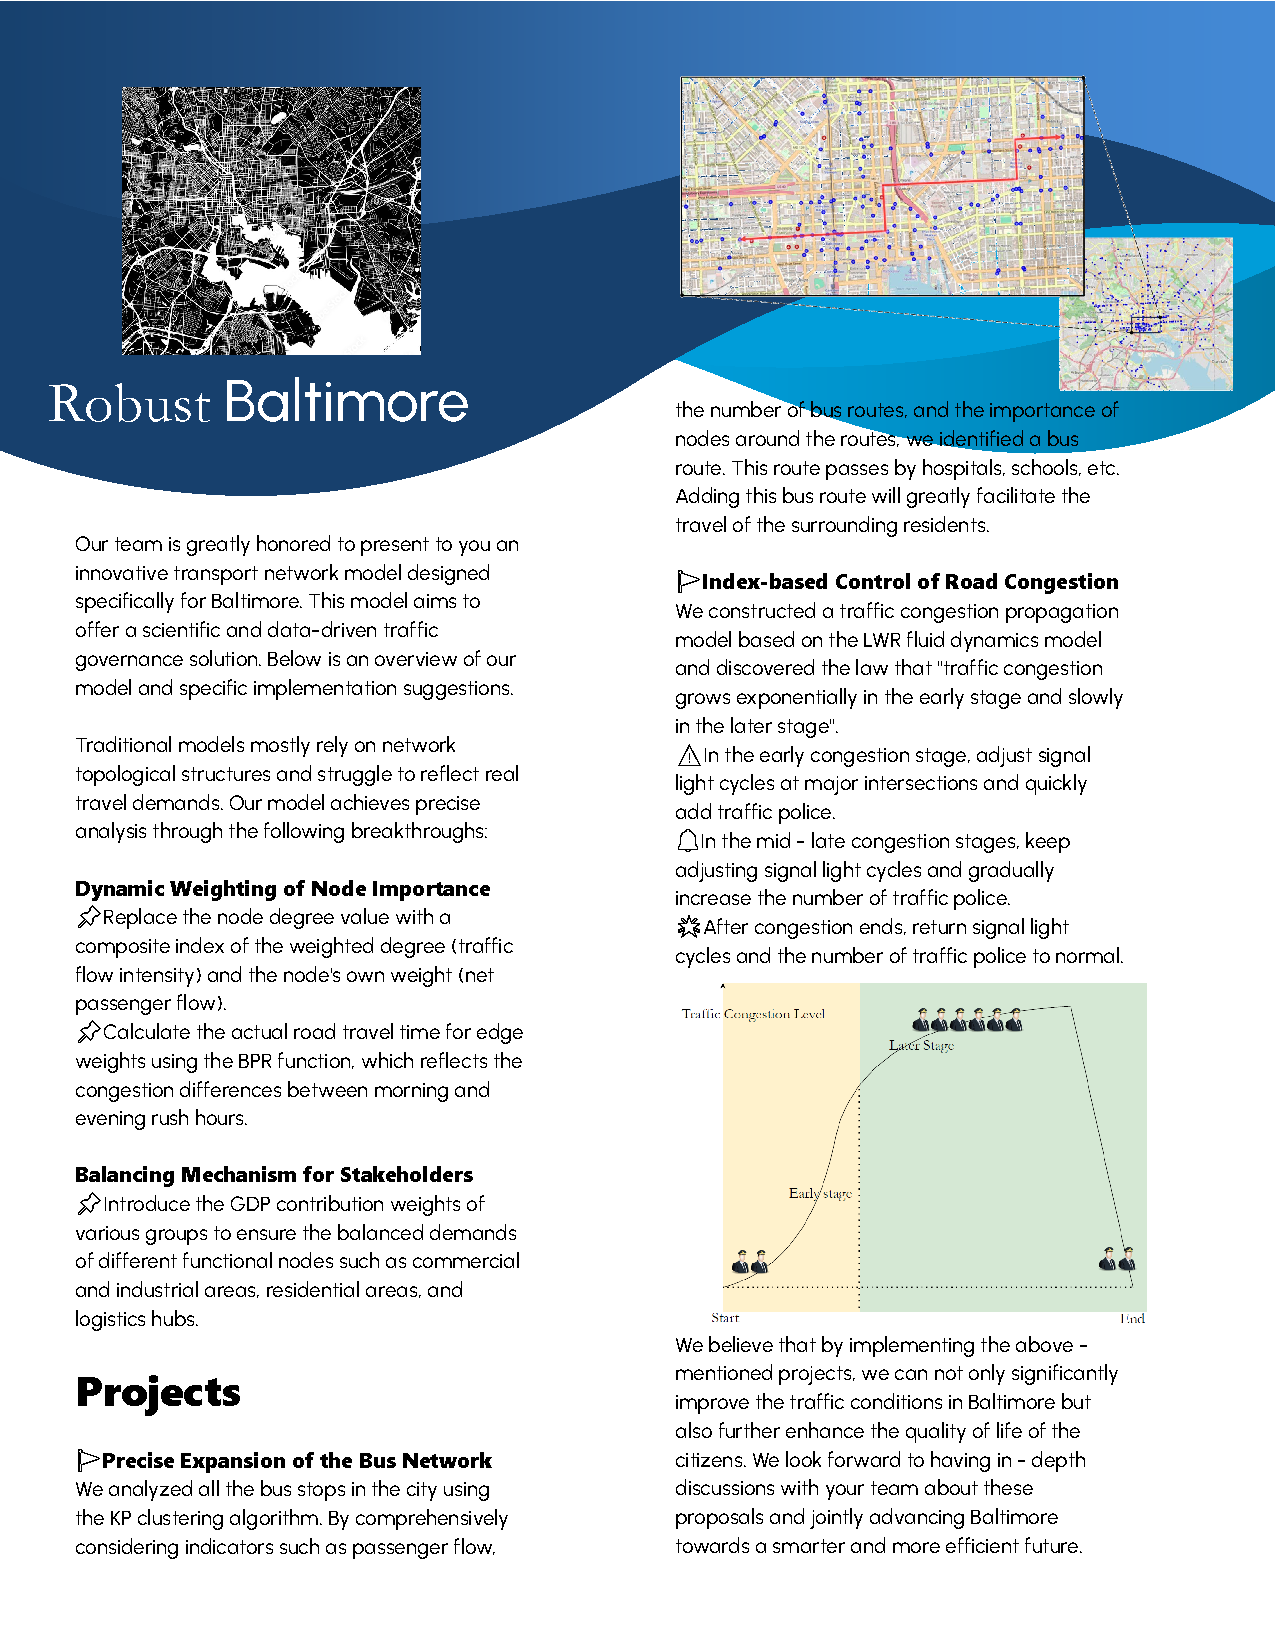
\includepdf[pages=-]{figures/letter.pdf}

\newpage
\section{引用文献}
\bibliographystyle{unsrt}
\bibliography{ref}
\newpage


\end{document}
